% Chapter 6

\chapter{Contribution and Discussion} % Chapter title

\label{ch:contribution} % For referencing the chapter elsewhere, use \autoref{ch:mathtest}

%---------------------------------------------------------------
While stratified PLPs systems, such as Problog, have been explored since
the early 2000s, research on PASP is a more recent focus of study,
with early works outside Sato's probabilistic semantics dating back to the
end of the first decade of the 21st century.

This historical context and the hardness of probabilistic inference
under the Stable Models semantics are the main reasons why more
efficient KC algorithms for compiling PASP programs require
development.

For the reasons mentioned above, the contribution that this work aims to propose
is the compilation of PASP programs under \textit{Credal} and \textsc{MaxEnt}
semantics that avoids introducing auxiliary variables during compilation,
taking inspiration from different works, as the bottom-up compilation
\citep{vlasselaer2014compiling} of Problog, the 2AMC framework for
probabilistic inference \citep{kiesel2022efficient, wang2025} and efficient encoding of
Pseudo-Boolean constraints (which are the case of cardinality constraints in
PASP) \citep{abio2012new}. Furthermore, this work also proposes a new
compilation paradigm for PLPs, called Non-Incremental compilation, where one
exploits the structure of the program to identify intertwined subsets of rules
that, when compiled independently, can be combined to form a more efficient
compilation, by taking inspiration from recent works on bottom-up compilation
\citep{de2023separating}.

\section{Formalization of the Proposal}

Previous studies in the field of KC suggest that, even
though SDDs are indeed less succinct than d-DNNFs,
the possibility of performing Boolean operations in polynomial
time is more than a sufficient trade-off in flexibility. This is
due to the fact that the \textit{Apply} operator in SDDs
enables direct compilation of program rules, avoiding the
introduction of auxiliary variables that may be inherent to
the Clark's completion procedure when using top-down compilers
\citep{vlasselaer2014compiling}.

In this sense, this work proposes bottom-up compilation
algorithms for compiling PASP programs into SDDs, in
order to perform both \textit{Credal} and \textsc{MaxEnt} inference,
described in Chapter \ref{ch:pasp}. This bottom-up compilation is
described in more depth in the following sections, where
structural constraints of the 2AMC problems are discussed.

Moreover, this work also claims that naive compilation of
circuits through the use of trivial initialization of the
\textit{V-tree} may not be sufficient to achieve satisfactory
results, as preliminary results suggest. Therefore, the
adaptation of a heuristic for initialization of $X$-constrained
$V$-tree is of great importance for the Answer Set Counting task, which is
the task of performing both \textit{Credal} and \textsc{MaxEnt} inference in
PASP. Although a heuristic may seem quite simple, it is still
relevant, since most state-of-the-art heuristics are focused on
CNF compilation; and do not leverage the structure of Probabilistic
Logic Programs.

Finally, to further enhance the compilation process, we propose an algorithm
that identifies disjoint components of the program (subsets of the program that
do not share any variables) in order to leverage theoretical properties that
ensure that the compilation process is linearly bounded by the size of the
intermediary representations of each one of these components. This approach
allows for more efficient compilation by focusing on smaller, independent
subproblems, which can be solved more quickly and with less memory overhead. If
the program cannot be decomposed into disjoint components, we reduce the
problem to a combinatorial optimization problem that can be solved efficiently,
in order to find a compromise that still enables us to leverage the theoretical
results of \citep{de2023separating}. This process is called Non-Incremental (bottom-up)
compilation and the algorithm described in \citep{de2023separating} assumed that
the decomposition of the formula was given, so this is the first work to
describe an algorithm that can decompose a program into disjoint components, in
such a way that the algorithm proposed in this work could be applied to any
other PLP; or even other target languages, such as And-Sum circuits
\citep{onaka2025and}, because they are also structured decomposable and share
the \textit{Apply} operator with SDDs.

\subsection{Class of Considered Programs}

This work focuses on ground PASP programs. This is a reasonable
consideration due to recent advancements in \textit{grounding} techniques for
Answer Set Programming. Thus, we do not consider the task of performing grounding in this
work, since it is a well-studied and optimized task in the literature
\citep{gebser2014clingo,gebser2016theory, kaminski2017tutorial}, so we assume
that the input program is already grounded.

There are also different considerations that could be made, such as assuming
that the input program is \textit{tight} (i.e. does not contain positive cycles
in the program dependency graph), because every \textit{non-tight} program can
be transformed into a tight one through the application of a technique called
\textit{cycle-breaking}, which is also a well studied topic in the literature
\citep{EITER2024104109}. Nevertheless, one interesting property of the bottom-up
compilation that has not been explored in depth in the literature is the fact
that it can leverage \textit{Loop Formulas} \citep{lee2003loop} to avoid the
need of using cycle-breaking to cope with positive cycles; and we will
explore this property in more detail in the following sections.

Finally, another consideration that is usually assumed when working with
PLPs that we will not assume is that the input program does have
\textit{annotated disjunctions}, i.e. usually it is assumed that the input
program only has \textit{probabilistic facts}. This assumption is usually
associated with the idea that the annotated disjunctions present in the
original program will undergo a transformation into probabilistic facts
\citep{shterionov2015most}. This transformation will not be covered in depth in
this work, since we will show how to cope with annotated disjunctions in a
similar way to cardinality constraints, as one can imagine annotated disjunction
as a cardinality constraint that imposes a \textit{exactly one} condition.

% This work is focused on PASP programs that fall into two
% different classes: \textit{tight} and \textit{head-cycle free}.
% This choice is motivated by the fact that both of them are
% highly expressive classes of programs, capable of representing
% \textit{non-stratification}, and can be easily transformed into
% CNF or Normal Logic Programs in polynomial time, as we
% describe after the following definitions.
%
% Furthermore, it is well known that the non-tight programs can
% be transformed into tight ones through the application of a
% transformation that is not covered in this work
% \citep{lee2003loop}.
%
% \begin{definition}[Tight Programs]
%     We say that a logic program $P$ is tight on a set $X$ of
%     literals if there is no infinite sequence $L_1, L_2, \ldots$
%     of elements of $X$ such that for every $i$, $L_{i+1}$ is a
%     parent of $L_i$ relative to $P$ and $X$
%     \citep{erdem2003tight}.
%
%     Moreover, a program $P$ is absolutely tight if satisfies:
%     there is no infinite sequence $L_1, L_2, \ldots$ of literals
%     such that for every $i$ there is a rule in $P$ for which
%     $L_{i+1}$ is a positive literal of the body and $L_i$ is
%     a head \citep{erdem2003tight}.
% \end{definition}
%
% One of the main advantages of restricting the class of programs
% to \textit{tight} (or \textit{absolute tight}) ones would be
% the possibility of easily generating CNF from the program,
% without the need of translating the program to a FOL
% theory, as we saw in the Clark's completion
% \citep{erdem2003tight}.
%
% \begin{definition}[HeadCycle-Free (HCF) Programs]
%     A logic program $P$ is HCF if and only if its
%     dependency graph $G$ does not contain a directed cycle going
%     through two head-sharing atoms in $P$
%     \citep{linke2004acyclic}.
% \end{definition}
%
% An interesting property of HCF programs is that they can be
% rewritten into Normal Logic Programs in polynomial time and space, via a
% technique called \textit{shifting} \citep{linke2004acyclic}.
% Therefore, besides this class of programs being highly
% expressible, they are also a useful framework for modeling
% ASP programs, since disjunctions in the head of rules can
% be transformed into regular rules from Normal Logic Programs
% \cite{linke2004acyclic}.
%
% \subsection{Some Considerations}
%
% Another well known transformation of PASP programs (and
% others PLPs), is the transformation of \textit{annotated
% disjunctions} into a series of probabilistic facts. The work
% of \citep{shterionov2015most} proposes building a
% \textit{Probability Tree}, a structure that encodes the
% probabilistic relation of an \textit{annotated disjunction} in
% a concise, flexible and modular way. For instance, consider
% Program \ref{lst:annotated_disjunction}, that has an annotated
% disjunction conditioned by a probabilistic fact $pick(b1)$.
% By encoding the annotated disjunction of size $n$ present in
% Program \ref{lst:annotated_disjunction} as a series of $n-1$
% mutually exclusive probabilistic facts, one is capable of
% representing the same probability distribution (Program
% \ref{lst:ad_tree}).
%
% \begin{listing}
%     \begin{lstlisting}
%         0.6::red(b1); 0.3::green(b1); 0.1::blue(b1) :- pick(b1).
%         0.6::pick(b1).
%     \end{lstlisting}
%     \caption{Example of Annotated Disjunction.}
%     \label{lst:annotated_disjunction}
% \end{listing}
%
% \begin{listing}
%     \begin{lstlisting}
%         0.6::pf(1, 1). 0.75::pf(1, 2).
%         red(b1):- pick(b1), pf(1, 1).
%         green(b1):- pick(b1), pf(1, 2), \+ pf(1, 1).
%         blue(b1):- pick(b1), \+ pf(1, 2), \+ pf(1, 1).
%         0.6::pick(b1).
%     \end{lstlisting}
%     \caption{PLP representing the Probabilistic Tree of Program \ref{lst:annotated_disjunction}.}
%     \label{lst:ad_tree}
% \end{listing}
%
% A similar simplification of the input programs is to replace
% \textit{probabilistic rules} with a new probabilistic fact,
% followed by its equivalent as a logic rule. For example, this
% transformation applied to Program  \ref{lst:probabilistic_rule}
% renders Program \ref{lst:probabilistic_rule_transformed}.
%
% \begin{listing}
%     \begin{lstlisting}
%         0.8::rain :- cloudy.
%     \end{lstlisting}
%     \caption{Example of Probabilistic Rule.}
%     \label{lst:probabilistic_rule}
% \end{listing}
%
% \begin{listing}
%     \begin{lstlisting}
%         0.8::rain_cloudy.
%         rain :- cloudy, rain_cloudy.
%     \end{lstlisting}
%     \caption{Result of transforming the Probabilistic Rule in Program \ref{lst:probabilistic_rule}.}
%     \label{lst:probabilistic_rule_transformed}
% \end{listing}
%
% Therefore, the input of our work is a ground PASP program
% that is \textit{tight} or \textit{head-cycle free} and does not
% have annotated disjunctions, since the transformation of these
% last can be easily performed by the user before the compilation.
%
% Furthermore, due to advances in \textit{grounding} techniques
% for ASP and PASP systems, we do not consider the task
% of performing grounding in this work, since it is a well studied
% and optimized task in the literature \citep{gebser2014clingo,
% gebser2016theory, kaminski2017tutorial}.
%
% One last consideration is that the input programs of our work,
% besides being ground and \textit{tight}/\textit{head-cycle
% free}, also had a \textit{cycle breaking} procedure applied to
% them. More specifically, we also consider the (positive)
% \textit{cycle-breaking} as one highly optimized task in the
% ASP literature, as treedwith aware algorithms for this task
% have been proposed by Eiter \citep{eiter2021treewidth}.
%
% Note that treewidth aware algorithms to perform Clark's
% completion also exist, but are not relevant to the methods
% explored in this work, since we focus on bottom-up compilation.
% On the other hand, this method will be considered in further
% experiments when comparing the performance of the proposed
% algorithms against top-down approaches, such as the ones
% explored by Eiter \citep{EITER2024104109}.

%---------------------------------------------------------------
\section{Motivation}

As a first consideration before approaching the PASP
compilation topic in more detail, it is important to note that
an enumerative approach to this problem can be consistently
better than a KC approach, but only if the number of
instances of the 2AMC problem to be solved is small
\citep{kiesel2022efficient}. More specifically, when considering
few probabilistic facts, the overhead of compiling the program
into a circuit representing its distribution is not amortized
over time, which can lead to a slower computation time when
compared to an enumerative approach. On the other hand, as one
can see by the work of \citep{kiesel2022efficient}, the KC
approach outperforms an enumerative approach when the number of
instances is significant.

This difference in performance is largely due to optimizations
of enumerative approaches that are not present in KC, such
as dynamic programming and caching \citep{gebser2014clingo,
gebser2016theory, kaminski2017tutorial} and other techniques
characteristic of ASP and \textsc{SAT} solvers
\citep{gong2017survey, toda2016implementing}.

Since this work revolves around the Neuro-Symbolic topic, which
encompasses the integration of Neural Networks with Probabilistic Logic Programming systems
through inference and learning algorithms \citep{geh2023dpasp,
manhaeve2018deepproblog,li2023scallop}, the KC approach
is best suited for the task at hand. The reason for this is that
learning algorithms are usually trained on large datasets and
 with a high number of iterations, which would make
the overhead of computing the 2AMC problem through a KC approach
amortized over time.

One great example to support this claim is the \textit{NeurASP}
system, which uses an enumerative approach to compute the \textit{Stable Models}
of a program. As the authors of the system stated, although this
naive approach of enumerating is highly competitive for small instances of
programs (few probabilistic facts), it is not scalable \citep{yang2023neurasp}.

%---------------------------------------------------------------
\section{Bottom-Up Compilation of PASP Programs}

In this first introduction to the compilation of PASP with
a bottom-up approach, we will describe how this algorithm
relates to the procedure of Clark's
Completion, with examples of how the compilation of rules that
have the same head can be performed in a more efficient way.

Furthermore, we present a naive approach to PASP
compilation, in order to hint at how an indiscriminate choice of
\textit{V-tree} initialization can lead to a circuit that does
not capture the structure of the program, if other
considerations (explained in the following sections) are not
taken into account.

\subsection{Relation to Clark's Completion}

In the previous literature review chapter
\ref{ch:literature_review}, the \textit{Clark's Completion} was
described in detail as a procedure to transform a Logic Program into
a CNF formula through the introduction of auxiliary
variables for heads of rules that appear more than once.

It is important to note that, even though this translation of
program to CNF formula is not particularly a difficult task
(since it only requires the applications of Equations
\eqref{eq:clark_cnf_1} and \eqref{eq:clark_cnf_2}, it does not take
advantage of the structure of the program. However, an obvious
but still a particularly interesting remark is that Logic Programs are not
CNF formulas. Since the CNF are a well-studied topic
for many applications, using it to encode knowledge can be
viewed as a rather straightforward approach, but it comes at
the cost of losing the structure of the program and introducing
unnecessary variables during compilation.

Finally, we note that we use a slightly different version of
Clark's completion, in order to obtain the boolean representation
of disjunctive programs, in Equation \eqref{eq:clark_completion_disjunctive}.
This completion can be seen as the result of applying the
\textit{Shifting} technique to the original PASP program
\citep{lee2003loop}.

\begin{equation}
    \textsc{Clark}(P) = \bigwedge_{a \in \mathcal{A}(P)}
    \left[a \iff \bigvee_{r \in \mathcal{R}(P,a)}
    \bigwedge_{b \in \textsc{body}(r)} b
    \bigwedge_{a' \in \textsc{head}(r) \setminus \{a\}} \neg a'
    \right].
    \label{eq:clark_completion_disjunctive}
\end{equation}

Note that Shifting can be viewed as a preprocessing step that
transforms a disjunctive program of the form Program
\ref{lst:pre_shifting} into Program \ref{lst:post_shifting}.
Hence, we will consider (from now on) that all input programs
to the compiler are already shifted; and, thus, their completion
is given by Clark's completion discussed in \ref{ch:literature_review}.

\begin{program}
    \begin{lstlisting}
    a; b :- c, d.
    \end{lstlisting}
    \caption{Example of a disjunctive program.}
    \label{lst:pre_shifting}
\end{program}

\begin{program}
    \begin{lstlisting}
    a :- c, d, not b.
    b :- c, d, not a.
    \end{lstlisting}
    \caption{Example of a disjunctive program after shifting.}
    \label{lst:post_shifting}
\end{program}

\subsection{Bottom-Up Compilation}

The bottom-up compilation is rather straightforward, leveraging
the \textit{Apply} operator to compile a succinct representation
of the program by following Equation \eqref{eq:clark_completion_disjunctive}.
The core idea of this approach consists in checking if an atom
appears as the head of multiple rules. If it is not the case,
then the compilation of the rule consists in applying an \textit{if
and only if} operation between the head atom and the conjunction
of the literals in the body of this unique rule. This process can
be seen in program \ref{lst:unique_head}, where the resulting
bottom-compilation is shown in Fig. \ref{fig:head_rule}.

\begin{program}
    \begin{lstlisting}
        turing :- godel, church.
    \end{lstlisting}
    \caption{Example of a program with an atom that appears as
    head only in one rule.}
    \label{lst:unique_head}
\end{program}

\begin{figure}
    \begin{center}
        \includegraphics[height=5cm]{../thesis/gfx/head_rule.pdf}
    \end{center}
    \caption{Compilation of Program \ref{lst:unique_head}
    to an SDD with balanced V-tree (with variable order as
    they appear in the program).}
    \label{fig:head_rule}
\end{figure}

In greater detail, the process of compiling the program
\ref{lst:unique_head} consists of the following steps:

\begin{enumerate}[label=(\roman*),ref=\roman*]
    \item Initializing a balanced V-tree, that the SDD
    will respect;
    \item Compiling each atom into an SDD representing
    the observation of the atom itself;
    \item Compiling the body of the rule into an SDD
    $\alpha$ by performing a conjunction of the literals in the
    body: $godel \land church$ (where $godel$ and $church$ here
    represent their respective SDD and $\land$ the
    conjoin operation);
    \item Performing an \textit{if and only if} operation
    between the previously obtained SDD $alpha$, from the
    conjoin operation, and the SDD of the head of the rule:
    $turing \iff \alpha$ (where $turing$ represents the
    SDD of the atom \textit{turing} and $\iff$ the Boolean
    \textit{if and only if} operation).
\end{enumerate}

If we have a program where the same atom appears as the head of
multiple rules, the process is slightly more complex, but still
intuitive. Differently from the CNF approach, where an
auxiliary variable would be introduced, the bottom-up
proceeds by compiling each body of the rules that have the same
head and performing a disjunction between the resulting
circuits. This can be seen as computing the $\vee$ operator
from Equation \eqref{eq:clark_completion}.

Consider the following program \ref{lst:multiple_head}, where
the atom $knuth$ appears as the head of two rules. To compile
such a program we first compile the bodies of the rules, with the
same approach as before, and then perform a disjunction between
all different bodies, resulting in a single circuit. Then, we
apply the \textit{if and only if} operation between the head of
rules and the circuit of the bodies, as we see in Figure
\ref{fig:multiple_head}.

Therefore, the single difference between the compilation of a
rule with a unique head and the compilation of a set of rules
with the same head is the disjunction operation between the
bodies of the rules. By applying this approach, we can avoid
the introduction of auxiliary variables, by utilizing the
\textit{apply} operation of SDDs.

\begin{program}
    \begin{lstlisting}
        knuth :- polya, church.
        knuth :- vonNeumann.
    \end{lstlisting}
    \caption{Example of a program with an atom that appears as
    head in multiple rules.}
    \label{lst:multiple_head}
\end{program}

\begin{figure}[bth]
    \centering
    \begin{subfigure}{0.25\linewidth}
        \centering
        \includegraphics[width=\linewidth]{../thesis/gfx/multiple_head_body.pdf}
        \caption{An SDD representing $polya \land church$.}
        \label{fig:multiple_head1}
    \end{subfigure}%
    \hfill
    \begin{subfigure}{0.65\linewidth}
        \centering
        \includegraphics[width=\linewidth]{../thesis/gfx/multiple_head.pdf}
        \caption{The result of the \textit{iff} operation between $knuth \iff (polya \land church) \lor vonNeumann$.}
        \label{fig:multiple_head3}
    \end{subfigure}
    \caption{Compilation of Program \ref{lst:multiple_head} into an SDD with balanced V-tree (with variable order as they appear in the program).}
    \label{fig:multiple_head}
\end{figure}

Summarizing, the bottom-up compilation of PASP programs
is defined as the following algorithm. Let $P$ be a PLP and
consider a predefined \textit{V-tree} initialization for the
SDD iterative compilation defined as follows:

\begin{enumerate}[label=(\roman*),ref=\roman*]
    \item Compile each atom of the propositional program $P$
    into an SDD representing the observation of the atom
    itself;
    \item For each atom $a$ that appears as a head of the
    program $P$:
    \begin{enumerate}
        \item For each rule $r$ that has $a$ as the head,
        compile the conjunction (by applying the
        \textit{conjoin} operator) of each literal in the body
        of $r$ (if an atom appears negated in the body, apply
        the $\neg$ operator to its respective SDD
        initialized in the first step);
        \item Perform a disjunction (by applying the
        \textit{disjoin} operator) between the resulting
        SDDs from the previous step.
    \end{enumerate}
    \item Apply an \textit{if and only if} operation between the
    SDD of the head of the rules and the resulting circuit
    from the disjunction of the bodies, from the previous step.
    \item Conjoin the resulting circuits of the previous step to
    obtain the circuit representing the program $P$.
\end{enumerate}

By analyzing the algorithm above, one can see that it also
correctly handles integrity constraints, as these can be seen
as an immediate consequence of the Clark's completion (Equation
\eqref{eq:clark_completion}). By considering the empty head of
integrity constraints as $false$; and solely following the steps
described in the bottom-up algorithm, we are able to correctly
compile the integrity constraints in a similar manner as
other normal rules.

Now, consider the Program\ref{lst:rule_by_rule}, where we combine rules
from Programs \ref{lst:unique_head} and \ref{lst:multiple_head}.
In this case, the compilation of the program, followed by
compiling first the rule where $turing$ is the head and then
the rules where $knuth$ is the head, would result in the circuit
described by Figure \ref{fig:rule_by_rule} (when considering a
balanced \textit{V-tree}, with variables appearing in the order
as they are presented in the program).

\begin{program}
    \begin{lstlisting}
        turing :- godel, church.
        knuth :- polya, church.
        knuth :- vonNeumann.
    \end{lstlisting}
    \caption{Example of a program with rules both from Programs
    \ref{lst:unique_head} and \ref{lst:multiple_head}.}
    \label{lst:rule_by_rule}
\end{program}

\begin{figure}
    \begin{center}
        \includegraphics[width=0.95\textwidth]{../thesis/gfx/rule_by_rule.pdf}
    \end{center}
    \caption{Compilation of the Program \ref{lst:rule_by_rule},
    obtained by application of the \textit{conjoin} SDD
    operator between the circuits of Figures \ref{fig:head_rule}
    and \ref{fig:multiple_head3}. Moreover, the \textit{V-tree}
    of the circuit is balanced, and the variables appear in the
    order they are presented in Program \ref{lst:rule_by_rule}.}
    \label{fig:rule_by_rule}
\end{figure}

A final, but extremely relevant, consideration is that, until now,
the bottom-up algorithm described only correctly represents
acyclic programs (programs without any positive cycles). This is
enough if one applies cycle-breaking as a pre-processing technique
in order to break positive cycles in the dependency graph of the
program. On the other hand, due to the flexibility of the
\textit{Apply} operator, it is easy to directly compile \textit{Loop
Formulas} without introducing auxiliary variables (as it is usually
done to avoid costly translations to CNF). More specifically,
for each loop $L$ in the positive dependency graph of a program $P$,
we have that its completion is given by:
\begin{equation}
    \label{eq:loop_formula}
    \text{Loop}(L) \equiv \bigvee_{l \in L} l \implies \bigwedge_{r \in R(L)}
    \bigwedge_{b \in body(r)} b \bigwedge_{a \in head(r) a \notin L} \neg a,
\end{equation}
where $R(L)$ is the set of rules that share a head with an atom inside
the loop $L$; and that do not share any body atoms with the atoms in $L$
\citep{lee2003loop}. This consideration concludes the bottom-up compilation
of disjunctive programs, thus leaving the compilation of cardinality
constraints as the only remaining challenge to address ASP compilation.

\subsection{Constraint Compilation}

Another key challenge in PASP compilation is the representation of
cardinality constraints. While there are well-studied methods in
the literature capable of encoding such constraints more succinctly,
such as Sequential Counters \citep{marques2007towards} and Totalizers
\citep{bailleux2003efficient}, they introduce auxiliary variables,
which our approach aims to mitigate. Thus, we propose a method to
compile an upper cardinality constraint by calling
$\text{Upper}(A, 0, u)$. This is an adaptation of \citep{abio2012new}
that leverages bottom-up compilation to avoid introducing auxiliary
variables:
\begin{equation}
    \label{eq:upper}
    \text{Upper}(A, c, t) = \begin{cases}
        \text{false}, & \text{if } c > t; \\
        \text{true}, & \text{if } |A| \le t - c; \\
        \textsc{ITE}(a, \text{Upper}(A \setminus \{a\}, c + 1, t), \text{Upper}(A \setminus \{a\}, c, t)), & \text{otherwise}.
    \end{cases}
\end{equation}
where $A$ represents the set of atoms inside the cardinality constraint,
$c$ is a counter of the current number of \emph{true} atoms at the time
of the function call, and $u$ is the upper value of the constraint. Even
though Equation \eqref{eq:upper} only encodes an upper cardinality constraint,
it is fairly straightforward to generalize it for a lower bound cardinality
constraint:

\begin{equation}
    \label{eq:lower}
    \text{Lower}(A, c, t) = \begin{cases}
        \text{true}, & \text{if } c \ge t; \\
        \text{false}, & \text{if } |A| + c < t \\
        \textsc{ITE}(a, \text{Lower}(A \setminus \{a\}, c + 1, t), \text{Lower}(A \setminus \{a\}, c, t)), & \text{otherwise}.
    \end{cases}
\end{equation}

With the above Equations \eqref{eq:lower} and \eqref{eq:upper}, we can encode
any cardinality constraint efficiently, whether it is an upper bound, a lower bound,
or a combination of both. On the other hand, ``exactly $k$'' constraints are of
special importance, particularly because annotated disjunctions can be seen as ``exactly one''
cardinality constraints. Usually, annotated disjunctions are encoded using a
method proposed by \citep{shterionov2015most}, which essentially encodes a
Sequential Counter \citep{marques2007towards} by introducing auxiliary variables.
However, by exploiting simple symmetries, we can combine both upper and lower
bounds into a single function that computes an ``exactly $k$'' constraint directly:

\begin{equation}
    \label{eq:exactly}
    \text{Exactly}(A, c, t) = \begin{cases}
        \text{false}, & \text{if } c > t \\
        \bigwedge_{a \in A} \neg a, & \text{if } c = t \\
        \text{false}, & \text{if } |A| + c < t \\
        \textsc{ITE}(a, \text{Exactly}(A \setminus \{a\}, c + 1, t), \text{Exactly}(A \setminus \{a\}, c, t), \text{false})
    \end{cases}
\end{equation}

Note that all of the above Equations \eqref{eq:upper}, \eqref{eq:lower}, and
\eqref{eq:exactly} can be easily generalized for the case of aggregators, when
each atom is associated with a weight, since they are quite flexible to encode
arbitrary pseudo-Boolean constraints.

In order to combine the compilation of the cardinality constraints into
our bottom-up approach, we just conjoin the results of the bottom-up compilation
with each circuit representing a cardinality constraint.

\subsection{Consideration About Succinctness}

Note that this approach is indeed more efficient than the one
that uses the Clark's completion, but only when considering the
number of variables in the circuit. The number of nodes (or
edges) produced by the SDD compiler is not necessarily
better than the one produced by the CNF compiler that uses
d-DNNFs, because the latter are able to compile formulas
more succinctly than the former Equation \eqref{eq:succinctness_hierarchy}.
Therefore, programs with a great number of rules with the same
head may not benefit greatly from this approach, but the
converse is also true, which means that the best approach
largely depends on the structure of the program.

%\subsection{Considerations About Structure of the Programs}
%
%The description of the bottom-up compilation algorithm
%indicates the advantages of restricting the scope of this work
%to \textit{tight} and \textit{head-cycle free} programs. The
%possibility of transforming ASP in Normal Logic Programs reduces
%the complexity of the compilation, since we do not have to
%consider programs with disjunctions in the head of the rules,
%something that would impose a great challenge to the previous
%defined algorithm.
%
%Besides imposing another operation the head of the rules,
%disjunction, there is a cardinality constraint associated with
%rules of this type \ref{ap:asp}. Hence, the compilation of
%cardinality constraints would be a great challenge to the topic
%of more general PASP compilation, but is also a great
%research opportunity, due to the expressive power of such type
%of rule.

\subsection{Limitations of Unconstrained Compilation}

As stated in the literature review \ref{ch:literature_review},
this algorithm is based on the work of
\citep{vlasselaer2014compiling}, in which the authors only
considered the compilation of \textit{stratified} programs, a
task that requires fewer constraints than the one proposed in this
work, since PASP programs are intrinsically related to the
notion of Answer Sets, as the name suggests.

This semantic difference between \textit{stratified} and
\textit{non-stratified} (PASP) programs is the main reason
for the development of this work, since the techniques proposed
for the former cannot be directly applied to the latter without
caution. The main reason for this is that the
\textit{stratified} does not encompass the \textit{Stable Model}
semantic, which is the main focus of the PASP programs.
When taking into account the \textit{Stable Model} semantics,
we will see (in the following sections) that a naive compilation
of a \textit{non-stratified} program. For example, Program
\ref{lst:hmm1}, with inference  performed by a circuit produced
by the bottom-up algorithm, can lead to erroneous results.

\begin{program}
    \begin{lstlisting}
        0.5::b(1).
        0.5::a(1).
        x(1) :- a(1).
        y(1,0); y(1,1) :- x(1).
        y(1,0) :- b(1), not x(1).
        y(1,1) :- not b(1), not x(1).
    \end{lstlisting}
    \caption{Example of a \textit{non-stratified} PASP
    program, representing a Hidden Markov Model.}
    \label{lst:hmm1}
\end{program}

% \begin{algorithm}
%     \caption{Bottom-Up Compilation via SDDs}
%     \label{alg:bottom-up}
%     \begin{algorithmic}[1]
%         \Require a \textit{ground} PASP program \(P\).
%         \Ensure An SDD representing the program \(P\).
%         \vspace{4pt}
%         \hrule
%         \vspace{4pt}
%         %
%         \Function{Bottom-Up SDD-Compilation}{$P$}
%         %
%         \State \(\Delta \gets \textsc{Initialize-V-Tree}(P)\)
%         %
%         \State \(\Sigma \gets \textsc{Initialize-SDD}(\Delta, \top)\)
%         %
%         \ForAll {\(h \in \textsc{heads(P)}\)}
%         %
%             \State \(\varphi \gets \textsc{Initialize-SDD}(\Delta, \bot)\)
%         %
%             \ForAll {\(r \in \textsc{Rules-with-Head}(P,h)\)}
%         %
%                 \State \(\psi \gets \textsc{Initialize-SDD}(\Delta, \top)\)
%         %
%                 \ForAll {\(b \in \textsc{bodies(r)}\)}
%         %
%                     \State \(\psi \gets \textsc{Conjoin}(\psi, b)\)
%         %
%                 \EndFor
%         %
%                 \State \(\varphi \gets \textsc{Disjoin}(\varphi, \psi)\)
%         %
%             \EndFor
%         %
%             \State \(\varphi \gets \textsc{IFF}(\varphi, h)\)
%         %
%             \State \(\Sigma \gets \textsc{Conjoin}(\Sigma, \varphi)\)
%         %
%         %
%         \EndFor
%         %
%         \State \ Return \(\Sigma\)
%         %
%         \EndFunction
%     \end{algorithmic}
% \end{algorithm}

For instance, Figure \ref{fig:hmm1} represents the results of
two different initializations of the \textit{V-tree} for the
bottom-up algorithm, using the program
\ref{lst:hmm1}, where Figure \ref{fig:hmm1_right} represents a
right-linear initialization and Figure \ref{fig:hmm1_left} a
left-linear initialization. Note that the results are different
in structure, number of nodes and edges, but both of them
retrieve the exact same number for Model Counting (MC). On the other hand,
this does not imply that both of them are able to correctly
compute the desired inferences for \textit{Credal} or
\textsc{MaxEnt}, since the structure of the circuit does not impose
any constraints on the variables, which can lead to erroneous
results for WMC tasks, if this is not taken into account
(a more detailed explanation of this problem is given in the
following sections).

\begin{figure}[bth]
    \centering
    \begin{subfigure}{0.45\linewidth}
        \centering
        \includegraphics[width=\linewidth]{../thesis/gfx/hmm_right.pdf}
        \caption{Bottom-Up compilation of the Program \ref{lst:hmm1} following a right-linear V-tree.}
        \label{fig:hmm1_right}
    \end{subfigure}%
    \hfill
    \begin{subfigure}{0.45\linewidth}
        \centering
        \includegraphics[width=\linewidth]{../thesis/gfx/hmm_left.pdf}
        \caption{Bottom-Up compilation of the Program \ref{lst:hmm1} following a left-linear V-tree.}
        \label{fig:hmm1_left}
    \end{subfigure}
    \caption{Bottom-Up compilation of the program \ref{lst:hmm1} by using
    bottom-up algorithm, using two different
    v-tree initializations: right-linear \ref{fig:hmm1_right}
    and left-linear \ref{fig:hmm1_left} (with variable order as
    they appear in the program).}
    \label{fig:hmm1}
\end{figure}

Therefore, we delve into the two main approaches to solve this
WMC problem when considering inference KC of
PASP programs.

\subsection{Preliminary Results}

In order to elucidate the impact of translating a program into
a CNF representing, Figure~\ref{fig:auxiliary} compares how
many auxiliary variables are needed to compile a program via its
Clark's completion, when one uses top-down compilation. The
datasets that are considered here are explained in detail in
Section~\ref{sec:experimental_results}.

\begin{figure}
  \centering
  \begin{subfigure}{0.48\linewidth}
    \centering
    \includegraphics[width=\linewidth]{../thesis/gfx/auxiliary_atoms/auxiliary_atoms_coloring.pdf}
    \caption{IRL}
    \label{fig:auxiliary_irl}
  \end{subfigure}
  \hfill
  \begin{subfigure}{0.48\linewidth}
    \centering
    \includegraphics[width=\linewidth]{../thesis/gfx/auxiliary_atoms/auxiliary_atoms_irn.pdf}
    \caption{IRN}
    \label{fig:auxiliary_irn}
  \end{subfigure}
  \vspace{0.5em}
  \begin{subfigure}{0.48\linewidth}
    \centering
    \includegraphics[width=\linewidth]{../thesis/gfx/auxiliary_atoms/auxiliary_atoms_coloring.pdf}
    \caption{Coloring}
    \label{fig:auxiliary_coloring}
  \end{subfigure}
  \hfill
  \begin{subfigure}{0.48\linewidth}
    \centering
    \includegraphics[width=\linewidth]{../thesis/gfx/auxiliary_atoms/auxiliary_atoms_coloring_complete.pdf}
    \caption{Coloring Complete}
    \label{fig:auxiliary_coloring_complete}
  \end{subfigure}
  \vspace{0.5em}
  \begin{subfigure}{0.48\linewidth}
    \centering
    \includegraphics[width=\linewidth]{../thesis/gfx/auxiliary_atoms/auxiliary_atoms_pin.pdf}
    \caption{PIN}
    \label{fig:auxiliary_pin}
  \end{subfigure}
  \hfill
  \begin{subfigure}{0.48\linewidth}
    \centering
    \includegraphics[width=\linewidth]{../thesis/gfx/auxiliary_atoms/auxiliary_atoms_pin_complete.pdf}
    \caption{PIN Complete}
    \label{fig:auxiliary_pin_complete}
  \end{subfigure}
  \vspace{0.5em}
  \begin{subfigure}{0.48\linewidth}
    \centering
    \includegraphics[width=\linewidth]{../thesis/gfx/auxiliary_atoms/auxiliary_atoms_food.pdf}
    \caption{Food}
    \label{fig:auxiliary_food}
  \end{subfigure}
  \hfill
  \begin{subfigure}{0.48\linewidth}
    \centering
    \includegraphics[width=\linewidth]{../thesis/gfx/auxiliary_atoms/auxiliary_atoms_queens.pdf}
    \caption{Queens}
    \label{fig:auxiliary_queens}
  \end{subfigure}
  \caption{Comparison of number of auxiliary variables introduced during Clark's completion
  across eight different datasets. The x-axis and y-axis represent, respectively, the size
  of the number of auxiliary variables and the instance size.}
  \label{fig:auxiliary}
\end{figure}

As one can see in Figure~\ref{fig:auxiliary}, in almost all datasets (besides \textsc{IRL}),
the number of auxiliary variables introduced during Clark's completion significantly
increases as the instance size grows. This suggests that the motivation behind this work is
a fair one: even though SDDs are proven to be less succinct than sd-DNNFs, the
large number of auxiliary variables introduced during Clark's completion suggests that
the bottom-up compilation can be a fair alternative to the state-of-the-art PASP
compilation.

%---------------------------------------------------------------
\section{PASP as a 2AMC problem}

The first approach that we consider is the 2AMC problem. This is a generalization of the
AMC problem, superficially described in the literature review
\ref{ch:literature_review} and described in more detail in the
\citep{kimmig2017algebraic, wang2025}. We highly recommend the
reader not familiarized with the WMC problem in general to read
\citep{kimmig2017algebraic} before continuing this section. In
summary, WMC is a framework that generalizes probabilistic inference over
propositional formulas with weighted atoms.

\subsection{Credal Semantics as an Instance of 2AMC}

As described in the preliminary Chapter \ref{ch:pasp}, the
Credal semantics is deeply related to the
notion of \textit{brave} and \textit{cautious reasoning}, in the
sense that we want to compute a probability interval
$[\underline{\mathbb{P}}(\mathcal{M}), \overline{\mathbb{P}}
(\mathcal{M})]$ (Equation \eqref{eq:credal_semantics}), for a set of models
$\mathcal{M}$, such that

$$
\overline{\mathbb{P}}(\mathcal{M}) = \sum_{\theta \in \Theta
: \Gamma(\theta) \cap \mathcal{M} \ne \emptyset} \mathbb{P}
(\theta), \qquad
\underline{\mathbb{P}}(\mathcal{M}) = \sum_{\theta \in
\Theta : \Gamma(\theta) \subseteq \mathcal{M}} \mathbb{P}
(\theta),
$$

where $\Theta$ is the set of all total choices, and $\Gamma
(\theta)$ the set of stable models associated with the
total choice \citep{cozman2017semantics, cozman2020joy}.

Although both equations above are not immediately recognizable
as an instance of the 2AMC problem, its characterization
as:

$$
\overline{\mathbb{P}}(\mathcal{M}) = \sum_{\theta \in \Theta}
\left[ \mathbb{P}(\theta) \cdot \bigwedge_{\gamma \in \Gamma(
\Theta)} [\![ \gamma \in \mathcal{M} ]\!] \right],
$$
$$
\underline{\mathbb{P}}(\mathcal{M}) = \sum_{\theta \in \Theta}
\left[ \mathbb{P}(\theta) \cdot \bigvee_{\gamma \in \Gamma(
\Theta)} [\![ \gamma \in \mathcal{M} ]\!] \right].
$$

Formally, one can see that the two semirings corresponding to
the upper probability interval in a 2AMC problem are:

\begin{itemize}
    \item The inner semiring $\mathcal{S}_I = (\set{0,1},
    \land, \land, \mathrm{true}, \mathrm{true})$, with labeling
    function $\alpha_I$ being constant as \textit{true} for all
    elements of the semiring;
    \item The outer semiring $\mathcal{S}_O = (\mathbb{R}_{\ge
    0}, +, \cdot, 0, 1)$, with labeling function $\alpha_O(o) =
    \mathbb{P}(o)$ for all elements of the semiring, which
    corresponds to the probability of a probabilistic fact $o$.
\end{itemize}

Furthermore, the weight transformation function can be
considered as the identity function, since it corresponds
elements with value $0$ from the inner AMC to $0$ in the
outer AMC, and the same is true for an inner AMC with
value $1$.

A similar approach can be taken for the lower probability, since
the main difference between both \textit{upper} and
\textit{lower} probabilities concerns the notion of
\textit{brave} and \textit{cautious} reasoning, respectively.
Moreover, by applying the ``tuple trick'' \citep{wang2025},
we can create semiring elements capable of representing the
computation of both \textit{upper} and \textit{lower}
probabilities at the same time, as an instance of the
2AMC problem.

\subsection{A Correct Property for 2AMC}

One of the main results of \citep{wang2025} regarding the 2AMC
problem is that both $X$-firstness and $X$-determinism are required
to efficiently compute inference in Answer Set Counting tasks (e.g., both
\textsc{MaxEnt} and the lower of \textit{Credal} semantics). In the context of
SDDs, we have that both properties coincide, rendering a
property called $X$-\textit{constrainedness}, defined as follows:

\begin{definition}[$X$-constrained]
    Let $V$ be a \textit{V-tree} and $v$ one of its nodes. We
    say that $v$ is $X$-constrained if and only if $v$ appears
    on the rightmost path of the \textit{V-tree} and $X$ is the
    set of variables outside $v$. Moreover, we say that a
    \textit{V-tree} is $X$-constrained if and only if it has an
    $X$-constrained.

    Finally, we say that an SDD is $X$-constrained if and
    if it is normalized for an $X$-constrained \textit{V-tree}.
    An SDD node is said to be $X$-constrained if and only
    if it is normalized for the $X$-constrained \textit{V-tree}
    node.
\end{definition}

Formally, the notion of $X$-\textit{constrained} is
characteristic of SDDs (more generally, SDNNFs), since
its definition is based on the notion of a \textit{V-tree}
respecting this order between partitions of variables. In the
case of sd-DNNFs this notion is not present, since they
do not need to respect the \textit{structured decomposability}
property \ref{ch:compilation}. However, one (strong) property
that can be imposed on sd-DNNFs that ensures tractability
of the 2AMC problem would be the variable decomposition
used in its construction. For example, the \textit{c2d} compiler
utilized the Shannon Decomposition, with some dynamic reordering
of the variables, which renders the resulting sd-DNNF the
desired property \citep{darwiche2004new}.

An important observation is that \citep{kiesel2022efficient}
claims that the $X$-\textit{firstness} property
\ref{ch:literature_review} by itself is indeed sufficient for the
tractable computation of the 2AMC problem over sd-DNNFs,
which is not true \citep{wang2025}, because such property is
neither \textit{necessary} nor \textit{sufficient} for a
tractable computation of the 2AMC problem. This mistake was
probably induced by the decomposition performed by the
\textit{c2d} compiler, which does not impose the
$X$-\textit{firstness}, but rather stronger properties
\citep{darwiche2004new} when performing variable decompositions.

On the other hand, $X$-\textit{determinism} is a property that
can be by itself \textit{sufficient} for efficient computation
of some of the desired inferences, such as the upper of the
\textit{Credal} semantics, more commonly known as \textit{MaxCredal}.

\subsection{2AMC Compilation via SDDs}

Note that, since the 2AMC task can be computed in
polynomial time through the use of an $X$-constrained V-trees,
by modifying the bottom-up algorithm to take into
account this type of structural constraint, we can compile a
PASP into a (smooth) SDD that is capable of computing
the 2AMC task in polynomial time. Hence, we are capable of
performing a bottom-up compilation of a PASP program into
a circuit that is capable of computing both \textit{Credal} and
\textsc{MaxEnt} queries in polynomial time, by restricting the
$V$-tree used in the bottom-up algorithm to be $X$-constrained
(i.e. the probabilistic variables are on the left of the $V$-tree;
while the logical variables are on the right).

% \subsection{Problems With This Approach}

% By enforcing the restriction of $X$-\textit{constrainedness} on
% SDDs, the search space for better \textit{V-trees} is
% largely reduced, which can lead to a poor performance of the
% algorithm. This is especially true for more complex programs,
% such as the \textit{Grid} and the \textit{HMM} family, in which
% sd-DNNFs were able to produce considerably more succinct
% circuits than SDDs, as can be seen in Table
% \ref{tab:preiliminary_results_opt}.

% \begin{table}
%     \makebox[1.15\textwidth][c]{
%         \begin{tabular}[c]{|c|c|c|c|c|c|c|c|c|c|}
%             \cline{2-9}
%             \multicolumn{1}{l|}{} & \multicolumn{4}{c|}{\textbf{SDD}} & \multicolumn{4}{|c|}{\textbf{sd-DNNF}} \\ \hline
%             \multicolumn{1}{|c|}{Program Name} & \#Nodes &
%             \#Edges & Time (s) & Cmpr. & \#Nodes & \#Edges &
%             Time (s) & Cmpr. & \#Models \\ \hline
%             \multicolumn{1}{|c|}{Simple} & $\mathbf{38}$ &
%             $\mathbf{53}$ & $3.42$ & $\mathbf{0.11}$ & $44$ &
%             $61$ & $\mathbf{0.004}$ & $0.09$ & $6$ \\ \hline
%             \multicolumn{1}{|c|}{Simple w/c} & $56$ & $84$ &
%             $3.18$ & $0.083$ & $\mathbf{51}$ & $\mathbf{76}$
%             & $\mathbf{0.005}$ & $\mathbf{0.09}$ & $7$ \\ \hline
%             \multicolumn{1}{|c|}{Montyhall} & $152$ & $236$ &
%             $3.28$ & $0.093$ & $\mathbf{124}$ & $\mathbf{181}$ &
%             $\mathbf{0.003}$ & $\mathbf{0.12}$ & $22$ \\ \hline
%             \multicolumn{1}{|c|}{Grid $3\text{-}3\text{-}3$} & $800899$ &
%             $1902593$ & $80.31$ & $42.38$ & $\mathbf{95757}$
%             & $\mathbf{205448}$ & $\mathbf{0.024}$
%             & $\mathbf{392.41}$ & $80621568$\\ \hline
%             \multicolumn{1}{|c|}{Latin Square $3\text{-}3$} &
%             $\mathbf{2764}$ & $\mathbf{6190}$ & $3.77$ & $7.54$
%             & $7929$ & $21353$ & $\mathbf{0.027}$ & $2.18$ &
%             $46656$ \\ \hline
%             \multicolumn{1}{|c|}{HMM$9$} & $13742$ & $27938$ &
%             $3.75$ & $46.92$ & $\mathbf{582}$ & $\mathbf{1031}$
%             & $\mathbf{0.007}$ & $1271.3$ & $1310720$ \\ \hline
%             \multicolumn{1}{|c|}{HMM$10$} & $31647$ & $64878$ &
%             $4.11$ & $96.97$ & $\mathbf{720}$ & $\mathbf{1338}$
%             & $\mathbf{0.007}$ & $\mathbf{4702.13}$ & $6291456$
%             \\ \hline
%             \multicolumn{1}{|c|}{HMM$15$} & $1421999$ &
%             $2901039$ & $33.47$ & $3146.05$ & $\mathbf{1275}$ &
%             $\mathbf{2548}$ & $\mathbf{0.009}$ &
%             $\mathbf{3581948.79}$ & $9126805504$
%             \\ \hline
%         \end{tabular}
%     }
%     \caption{Prelimniary results of the compilation of PASP
%     programs using $X$-\textit{constraint} SDDs respecting
%     a balanced V-tree initialization, when compared to
%     sd-DNNFs (compiled via \textit{c2d}) that follows a
%     (static) heuristic for its variable decomposition.}
%     \label{tab:preiliminary_results_opt}
% \end{table}

% One of the main advantages of sd-DNNFs in this context was
% the introduction of a heuristic that is capable of producing a
% better variable decomposition than the one obtained by the
% naive application of the $X$-\textit{constraint} over the
% variables. This hints one of the proposed improvements for this
% work, which is the adaptation of well-studied heuristics for
% SDDs to the PASP compilation task, in order to
% exploit the full potential of this type of circuit.

% However, careful considerations about these results must be
% taken into account. As discussed in the previous paragraph,
% following a property such as the $X$-\textit{constraint} can be
% highly detrimental to the succinctness of the circuit, as one
% is not able to explore the full potential of the possible
% \textit{V-trees} that can be used to compile the program.

% As we are going to see in the following sections, there are
% alternative approaches that can be taken to solve the PASP
% inference problem, which is closely related to the work of
% \citep{totis2023smproblog} (using unrestricted circuits, but
% leveraging recent discoveries for efficiently re-structuring
% circuits).

\subsection{Comments on Other Compilers}

The most popular approach to solve the 2AMC via KC in
recent works, such as \citep{EITER2024104109,
kiesel2022efficient}, encompasses the use of \textsc{c2d}
\citep{darwiche2004new}, \textsc{d4} \citep{lagniez2017improved}
and \textsc{SharpSAT} \citep{korhonen2021integrating} as knowledge
compilers. Indeed, the performance of these compilers can be rather
remarkable when compared to other top-down approaches \citep{EITER2024104109},
specially when considering the compilers that do not use d-DNNFs,
such as OBDDs-based compilers (such as \textit{CUDD}
\citep{somenzi1998cudd}, or \textit{BDDC} \citep{lai2017new}),
or even SDDs-based compilers (for example, \textit{miniC2D},
a variant of \textit{c2d} that compiles formulas into SDDs
instead of d-DNNFs) \citep{lai2022ccdd}.

More recent work even proposes a new language for representing
circuits, Constrained Conjunction and Decision Diagram (CCDD),
and gives birth to a new compiler, called
\textit{Panini} \citep{lai2022ccdd}, which surpasses the
performance of the previously mentioned compilers in a variety
of tests \citep{lai2022ccdd}.

An important note is that the results of
\citep{kiesel2022efficient} describe the ability of
sd-DNNFs of computing the 2AMC problem tractably.
Although this result immediately implies that
SDDs (and consequently, OBDDs) are capable of
performing the same task in polynomial time w.r.t the size of the
circuit, it is not clear if the same results follow for
CCDDs.

Moreover, even though the 2AMC problem can be solved by
sd-DNNF, \textit{smoothness} is not the only property that
circuits inside the d-DNNF family must have. As
mentioned before, the circuit must exhibit a structure alike
the $X$-\textit{constraint} property of SDDs in order to
perform such computational tasks tractably. With this problem
in mind, \textit{c2d} is the usual choice for solving 2AMC
tasks for PASP applications, due to the software's ability
ensuring structural constraints over the circuits it produces
(a task that is not trivial to ensure for other compilers).
On the other hand, both \textsc{d4} and \textsc{SharpSAT-TD}
were adapted by \citep{EITER2024104109} to ensure the necessary
structural constraints over the circuits they produce.

This implementation and algorithmic problem (concerning the
variable decomposition) are major bottlenecks for the usage of
sd-DNNF for compilation; and not only for PASP, but
also for CNF formulas in general. As we are going to see
in later sections, the possibility of dynamically reordering the
variables during a bottom-up compilation is a major advantage of
SDDs over sd-DNNFs, and can lead to a more succinct
circuit representation of the program (even though the
succinctness of the former is in a lower hierarchy than the
latter \eqref{eq:succinctness_hierarchy}). This approach is of
special interest when the input of the compilation is not a
program, where the structure can be exploited, but a CNF,
which is a common input for knowledge compilers.

\subsection{Preliminary Results}

Now, we delve into the first experimental results that indicate
how the bottom-up compilation via SDDs can be an interesting
alternative to the current state-of-the-art top-down compilation.
In Figure~\ref{fig:2amc}, we can see that even without using
any clever $V$-tree initialization, reordering or other techniques,
some of the most complex classes of programs, \textsc{PIN-Complete}
and \textsc{Queens}, are leveraged by the bottom-up compilation.
This are two classes of programs that are heavily impacted by the
increase of auxiliary variables (Figure~\ref{fig:auxiliary}).
Moreover, the bottom-up compilation had a fair performance on the
\textsc{IRL} dataset, largely surpassing \textsc{SharpSAT-TD} and
achieving comparable performance w.r.t. both \textsc{C2D} and\
\textsc{D4}. In the remaining datasets, performance of the bottom-up
compilation was poor, but we investigate, in the following sections,
improvements to the bottom-up compilation process that will flip
this situation, making it more competitive with the current
state-of-the-art.

\begin{figure}
  \centering
  \begin{subfigure}{0.48\linewidth}
    \centering
    \includegraphics[width=\linewidth]{../thesis/gfx/2amc/2amc_irl.pdf}
    \caption{IRL}
    \label{fig:2amc_irl}
  \end{subfigure}
  \hfill
  \begin{subfigure}{0.48\linewidth}
    \centering
    \includegraphics[width=\linewidth]{../thesis/gfx/2amc/2amc_irn.pdf}
    \caption{IRN}
    \label{fig:2amc_irn}
  \end{subfigure}
  \vspace{0.5em}
  \begin{subfigure}{0.48\linewidth}
    \centering
    \includegraphics[width=\linewidth]{../thesis/gfx/2amc/2amc_coloring.pdf}
    \caption{Coloring}
    \label{fig:2amc_coloring}
  \end{subfigure}
  \hfill
  \begin{subfigure}{0.48\linewidth}
    \centering
    \includegraphics[width=\linewidth]{../thesis/gfx/2amc/2amc_coloring_complete.pdf}
    \caption{Coloring Complete}
    \label{fig:2amc_coloring_complete}
  \end{subfigure}
  \vspace{0.5em}
  \begin{subfigure}{0.48\linewidth}
    \centering
    \includegraphics[width=\linewidth]{../thesis/gfx/2amc/2amc_pin_best.pdf}
    \caption{PIN}
    \label{fig:2amc_pin}
  \end{subfigure}
  \hfill
  \begin{subfigure}{0.48\linewidth}
    \centering
    \includegraphics[width=\linewidth]{../thesis/gfx/2amc/2amc_pin_complete_best.pdf}
    \caption{PIN Complete}
    \label{fig:2amc_pin_complete}
  \end{subfigure}
  \vspace{0.5em}
  \begin{subfigure}{0.48\linewidth}
    \centering
    \includegraphics[width=\linewidth]{../thesis/gfx/2amc/2amc_food_best.pdf}
    \caption{Food}
    \label{fig:2amc_food}
  \end{subfigure}
  \hfill
  \begin{subfigure}{0.48\linewidth}
    \centering
    \includegraphics[width=\linewidth]{../thesis/gfx/2amc/2amc_queens.pdf}
    \caption{Queens}
    \label{fig:2amc_queens}
  \end{subfigure}
  \caption{Comparison of circuit size for the different (top-down and bottom-up) compilers
  across eight different datasets. The x-axis and y-axis represent, respectively, the size
  of the circuit produced by a compiler and the instance size. Cyan, magenta, yellow, and
  black represent, respectively: \textsc{c2d}, \textsc{d4}, \textsc{SharpSAT-TD} and
  the bottom-up SDD compiler. Datasets where the black dots are consistently under the
  other colors representing scenarios where the bottom-up SDD compiler is more efficient;
  and vice versa.}
  \label{fig:2amc}
\end{figure}

%---------------------------------------------------------------
\section{V-tree Optimization}

Before delving into the second approach for PASP compilation,
which uses unrestricted $V$-trees, we discuss the impact of
$V$-tree initialization and reordering during the compilation
process.

% \subsection{An Elucidative Example}

% The \textit{structured decomposability} property of SDDs
% can be highly beneficial, when compared to sd-DNNFs,
% because it allows one to compute binary operations, such as
% \textit{conjoin} in polynomial time, instead of exponential time
% \citep{darwiche2004new, Darwiche_2002}. Although this property
% highly increases the expressiveness of functions that can be
% applied to SDDs, it also imposes such structures to follow
% \textit{V-trees}, which can deeply affect the size of circuit,
% depending on the structure of this variable tree
% \citep{darwiche2011sdd}. Thus, the choice of a good variable
% tree is akin to the choice of a good variable ordering in
% BDDs, in the sense that it can lead to a more succinct (or
% exponential larger) circuit representation of the compiled
% formula.

% Table \ref{tab:vtree_comparison} shows the results of compiling
% a program using different variable tree structures, such as
% \textit{balanced}, \textit{right-linear} and \textit{random}.
% The importance of this choice is evident, because both
% \textit{balanced} and \textit{right-linear} variable trees
% follow the $X$-\textit{constraint} property, necessary to
% perform the 2AMC task in polynomial time; with special
% importance to the \textit{right-linear} tree, which renders the
% SDD the same structure as a BDD. However, the
% \textit{random} tree does not follow this property in
% particular, but their sizes are particularly interesting, since
% larger instances of the \textit{HMM} family have an extremely
% small circuit representation when compared to the other
% \textit{V-trees}.

% This result of Table \ref{tab:vtree_comparison} only highlights
% the importance of the choice of a good variable tree for the
% circuit compilation. More over, it calls into question if
% imposing the $X$-\textit{constraint} over the variables is
% worth the trade-off of restricting its structure, which can
% lead to a less succinct circuit representation. This is of
% particular interest when one considers the possibility of
% following a similar approach to the one of \textit{smProblog},
% where the normalization step is intractable due to the
% computation of the total choices of the circuit, but the circuit
% itself is not restricted to a particular \textit{V-tree}
% structure.

% \begin{table}
%     \makebox[0.85\textwidth][c]{
%         \begin{tabular}[c]{|c|c|c|c|c|c|c|c|c|}
%             \hline
%             \multicolumn{3}{|c|}{\textbf{Balanced}} & \multicolumn{3}{|c|}{\textbf{Right-Linear}} & \multicolumn{3}{|c|}{\textbf{Random}} \\ \hline
%             \#Nodes & \#Edges & Time (s) & \#Nodes & \#Edges & Time (s) & \#Nodes & \#Edges & Time (s) \\ \hline
%             38 & 53 & 3.27 & \textbf{34} & \textbf{44} & \textbf{3.09} & 59 & 87 & 3.3 \\ \hline
%             \textbf{56} & \textbf{84} & \textbf{3.11} & 59 & 86 & 2.95 & 57 & 82 & 3.04 \\ \hline
%             152 & 236 & 3.27 & 203 & 328 & \textbf{3.10} & \textbf{34} & \textbf{45} & 3.25 \\ \hline
%             800899 & 1902593 & 77.60 & 2757555 & 5514810 & 111.63 & \textbf{800899} & \textbf{1902593} & \textbf{76.10} \\ \hline
%             \textbf{2764} & \textbf{6190} & 3.55 & 10184 & 20236 & \textbf{3.38} & 24999 & 59368 & 5.92 \\ \hline
%             13742 & 27938 & 3.65 & 26419 & 52654 & \textbf{3.54} & \textbf{3708} & \textbf{8149} & 4.91 \\ \hline
%             \textbf{31645} & \textbf{64878} & 4.08 & 76132 & 152064 & \textbf{4.02} & 159563 & 380288 & 23.21 \\ \hline
%             1421999 & 2901039 & 33.08 & 3408748 & 6817196 & 43.05 & \textbf{4898} & \textbf{10282} & \textbf{3.75} \\ \hline
%         \end{tabular}
%     }
%     \caption{Comparison of the number of nodes, edges and time
%     taken to compile the PASP programs of Table
%     \ref{tab:preiliminary_results} (appearing in the same order)
%     into SDDs using different variable tree structures:
%     \textit{balanced}, \textit{right-linear} and
%     \textit{random}.}
%     \label{tab:vtree_comparison}
% \end{table}

\subsection{Static Initialization of V-trees}

Problems related to \textit{structured decomposability} were
known even before the work of Darwiche when he proposed
SDDs \citep{pipatsrisawat2008new, darwiche2011sdd}. With
this in mind, Darwiche proposed some heuristics to initialize
SDDs \textit{V-trees} in a way that tries to minimize the
growth of the circuit during the compilation process, after
many conjoin and disjoin operations.

Hence, two methods for better initialization of \textit{V-trees}
were proposed in the paper that introduced SDDs:
\textit{minfill} and \textit{MINCE} \citep{darwiche2011sdd}. The
former adapts another heuristic proposed by Darwiche for
DNNFs \citep{darwiche2001decomposable}, exchanging the
roles of clauses and variables, and use the \textit{minfill}
heuristic for variable elimination, while still ensuring that
the leftmost child of a \textit{V-tree} node is always the one
with the smallest number of children. The latter, on the other
hand, is a heuristic that generates a variable ordering, which
is not as desirable as the one generated by \textit{minfill},
since the constraint of using a right-linear \textit{V-tree} is
basically enforcing a BDD structure. A possible
modification to this method, proposed by Darwiche, would be to
use a balanced or random \textit{V-tree}, obtained from the
variable ordering generated by \textit{MINCE}; but the results
were not as promising as the ones obtained by \textit{minfill}
\citep{darwiche2011sdd}.

Although both of these methods are interesting, they do not take
advantage of the program structure, i.e. they were developed for
CNF-based (top-down) approaches. By cleverly exploiting the
program structure, we can achieve better results, as we show soon.

The heuristic proposed in this work is quite simple: represent
the dependency graph of the program, count the number of descendants
of each node (reachable nodes, using a depth-first search), and use
this information to guide the construction of the \textit{V-tree}.
We expect that nodes with a high number of descendants ``imply''
in many other nodes, and thus they should appear early in the
\textit{V-tree}. For example, we have Figure~\ref{fig:dependency_graph}.

\begin{figure}
    \centering
    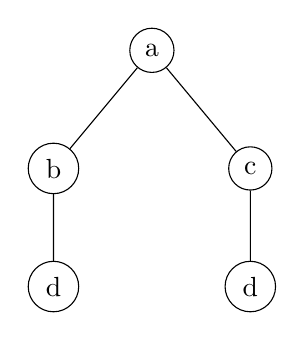
\begin{tikzpicture}[level distance=1.5cm, sibling distance=2.5cm, every node/.style={circle, draw}]
        \node (a) {a}
            child {node (b) {b}
                child {node (d1) {d}}
            }
            child {node (c) {c}
                child {node (d2) {d}}
            };
    \end{tikzpicture}
    \caption{Dependency graph of the program.}
    \label{fig:dependency_graph}
\end{figure}

Using this topological ordering, we can construct the \textit{V-tree}
that has on its left nodes with a high number of descendants and on its
right leaves of the dependency graph. As we show in Section \ref{sec:experimental_results},
this approach vastly improves the performance of the compilation process,
outperforming both \textsc{MinFill} and \textsc{MinDegree}.

\subsection{Dynamic Reordering of V-trees}

Alone, the approach of initializing the \textit{V-tree} with a
good heuristic is indeed promising, but it is well known that
compilation is indeed a hard task. If not, many well-known hard
Computer Theoretical problems could be associated with different
complexity classes.

Due to the hardness of the compilation task, it is expected that
eventual blow-ups in the size of the circuit will happen, so it
is only natural to think about a dynamic reordering of the
circuit, in order to keep the circuit as small as possible,
while not wasting too much time in the reordering process
itself.

With this in mind, the work of \citep{choi2013dynamic}
proposes two different heuristics for
dynamic re-ordenation, based on the concept of reordering the
variables of an OBDD \citep{rudell1993dynamic}. The
proposal of \citep{choi2013dynamic} is to reorder the structure of
an SDDs by the application of \textit{rotations} and
children \textit{swap}, but initially did not cover
$X$-constrained $V$-trees. This extension was proposed soon
after in \citep{oztok2016solving}.

This approach has achieved great success in the context of
compiling PLPs, since the work of
\citep{vlasselaer2014compiling}, when compiling rules directly
into SDDs, achieved a better performance with dynamic
reordering of the \textit{V-tree}. The circuit obtained by this
approach did not only have a considerably smaller size, but also
did not take too much time to be compiled, when compared to
their static counterpart.

\subsection{Heuristic-Based PASP Compilation}

By combining both static and dynamic approaches heuristics to
initialize and reorder the variable tree of the SDD,
during the compilation process, we can obtain algorithms for
enhancing the previously described methods for PASP
compilation. For instance, compilation like the one of
\textit{smProblog} is able to take advantage of an unrestricted
search space for the \textit{V-tree} initialization or
reordering, which could render a more succinct circuit,
analogous to the results of
\citep{vlasselaer2014compiling} (that took advantage of the
dynamic reordering of the variable tree to obtain considerably
smaller circuits for PLP programs, when compared to
methods without dynamic reordering). On the other hand, the
2AMC approach with $X$-\textit{constraint} (or even
$X$-determinism) needs the development of new heuristics, that
preserve a good variable ordering, while not disrespecting the
desired constraints over the circuit.

In order to combine these two improvements for the $V$-tree
during the bottom-up compilation, one simply needs to call
the heuristic when selecting the $V$-tree that will be fed
to the bottom-up algorithm and to apply dynamic reordering
of the variable tree when the SDD's size surpasses a certain
threshold, as described \citep{choi2013dynamic}. For example,
one could call the dynamic reordering when the SDDs size
doubles.

\subsection{Preliminary Results}

In this section, we focus on two different aspects: the impact of
using the proposed heuristic for $V$-tree initialization and the
impact of dynamic reordering on the bottom-up compilation. For the
$V$-tree initialization, we considered a slightly different version
of the \textsc{Coloring} dataset, where random graphs increase at
an lower rate, in order to capture the behavior of the different
heuristics across different graph sizes. Accordingly,
Table \ref{tab:vtree-comparison} shows that the proposed heuristic
outperforms the other two heuristics, both in terms of memory usage
and circuit size, highlighting the importance of considering program
structure when compiling PLPs, as opposed to other top-down
CNF-based approaches.

\begin{table}
    \centering
    \begin{tabular}{crrrrrr}
        \toprule
        \multirow{2}{*}{\#Nodes} & \multicolumn{2}{c}{Ours} & \multicolumn{2}{c}{MinDegree} & \multicolumn{2}{c}{MinFill} \\
        & mb & s & mb & s & mb & s \\
        \midrule
        %12 & \textbf{272} & \textbf{0.72} & 1608 & 6.91 & 385 & 1.17 \\
        13 & \textbf{374} & \textbf{2.42} & 10020 & 229 & 805 & 4.07 \\
        14 & \textbf{387} & \textbf{5.48} & - & - & 754 & 7.21 \\
        15 & \textbf{997} & 32.2 & - & - & 2939 & \textbf{31.99} \\
        16 & \textbf{9640} & \textbf{279} & - & - & - & - \\
        17 & \textbf{10411} & \textbf{588} & - & - & - & - \\
        \bottomrule
    \end{tabular}%
    \caption{Comparison of memory (\textbf{mb}) and time (\textbf{s}econds) between the proposed
    heuristic, MinDegree and MinFill for $V$-tree initialization in the \textbf{Coloring} dataset
    for bottom-up compilation.}
    \label{tab:vtree-comparison}
\end{table}

While $V$-tree initialization has its importance in order to provide a good
start for generating succinct circuits, dynamic reordering is one of the
most interesting aspects of bottom-up compilation, since it provides the
possibility of exploring different variable orderings during compilation.
Usually, when using top-down compilation, one chooses a variable ordering and
stays with it during all compilation steps; thus, dynamic reordering provides
a sound way to circumvent possible issues with the chosen ordering. Figure~\ref{fig:vtree}
shows how this dynamic reordering can be used to surpass top-down approaches on
some of the datasets that the previous section had poor performance, such as
\textsc{IRN} and \textsc{Food}. In the \textsc{Food} dataset, dynamic reordering
was essential to significantly improve the performance of bottom-up compilation.

\begin{figure}
  \centering
  \begin{subfigure}{0.48\linewidth}
    \centering
    \includegraphics[width=\linewidth]{../thesis/gfx/V_tree/Vtree_irl.pdf}
    \caption{IRL}
    \label{fig:vtree_irl}
  \end{subfigure}
  \hfill
  \begin{subfigure}{0.48\linewidth}
    \centering
    \includegraphics[width=\linewidth]{../thesis/gfx/V_tree/Vtree_irn.pdf}
    \caption{IRN}
    \label{fig:vtree_irn}
  \end{subfigure}
  \vspace{0.5em}
  \begin{subfigure}{0.48\linewidth}
    \centering
    \includegraphics[width=\linewidth]{../thesis/gfx/V_tree/Vtree_coloring.pdf}
    \caption{Coloring}
    \label{fig:vtree_coloring}
  \end{subfigure}
  \hfill
  \begin{subfigure}{0.48\linewidth}
    \centering
    \includegraphics[width=\linewidth]{../thesis/gfx/V_tree/Vtree_coloring_complete.pdf}
    \caption{Coloring Complete}
    \label{fig:vtree_coloring_complete}
  \end{subfigure}
  \vspace{0.5em}
  \begin{subfigure}{0.48\linewidth}
    \centering
    \includegraphics[width=\linewidth]{../thesis/gfx/V_tree/Vtree_pin_best.pdf}
    \caption{PIN}
    \label{fig:vtree_pin}
  \end{subfigure}
  \hfill
  \begin{subfigure}{0.48\linewidth}
    \centering
    \includegraphics[width=\linewidth]{../thesis/gfx/V_tree/Vtree_pin_complete_best.pdf}
    \caption{PIN Complete}
    \label{fig:vtree_pin_complete}
  \end{subfigure}
  \vspace{0.5em}
  \begin{subfigure}{0.48\linewidth}
    \centering
    \includegraphics[width=\linewidth]{../thesis/gfx/V_tree/Vtree_food_best.pdf}
    \caption{Food}
    \label{fig:vtree_food}
  \end{subfigure}
  \hfill
  \begin{subfigure}{0.48\linewidth}
    \centering
    \includegraphics[width=\linewidth]{../thesis/gfx/V_tree/Vtree_queens.pdf}
    \caption{Queens}
    \label{fig:vtree_queens}
  \end{subfigure}
  \caption{Comparison of circuit size for the different (top-down and bottom-up with dynamic
  reordering) compilers across eight different datasets. The x-axis and y-axis represent,
  respectively, the size of the circuit produced by a compiler and the instance size. Cyan,
  magenta, yellow, and black represent, respectively: \textsc{c2d}, \textsc{d4}, \textsc{SharpSAT-TD}
  and the bottom-up SDD compiler with dynamic reordering. Datasets where the black dots
  are consistently under the other colors representing scenarios where the bottom-up SDD
  compiler is more efficient; and vice versa.}
  \label{fig:vtree}
\end{figure}

It is also important to note that dynamic reordering comes at a cost, as it requires additional
computation time and resources to explore better $V$-trees during compile time. Although this
can be more granularly fine-tuned during compilation, we observed that this approach hurts
performance on some cases, such as \textsc{PIN Complete}, where this reordering overhead broke
the time wall of 30 minutes and made it impossible to compile the instance of size 6 under the
time limit.

%---------------------------------------------------------------
\section{Relaxing Constraints for PASP Compilation}

In this section, we comment on the work of \citep{totis2023smproblog} for the
\textit{smProblog} system, since both PASP and \textit{smProblog}
share the \textit{Stable Model} and \textsc{MaxEnt} semantics, but with one key
difference: the \textit{smProblog} allows for \textit{inconsistencies} in the
program, while this do not consider this possibility in PASP. This
difference is crucial, since the enumeration step of the \textit{Stable Models}
will not be the same, as all total choices will have at least one model in
PASP, while this is not necessarily true for \textit{smProblog}.

By taking inspiration from this unconstrained approach of \citep{totis2023smproblog},
we propose an alternative compilation method that leverages recent discoveries
in $V$-tree restructuring \citep{zhang2025}.

\subsection{Particularities of the smProblog System}

Another key detail of the \textit{smProblog} system is the usage
of the \textit{d-Sharp} knowledge compiler, described in the
previous section. While this may seem as like a minor detail, the
implementation of \textit{d-Sharp} does not allow for the
imposition of the $X$-\textit{firstness} or $X$-\textit{determinism} over the
circuit. Thus, need for an intractable normalization step by enumerating all
\textit{Stable Models} of the program is necessary.

This choice, although small, is one of the key arguments for the
usage of SDDs, since one is not locked by specific design
implementations of the knowledge compiler, and can both choose
the \textit{V-tree} initialization and check for properties as
$X$-\textit{constraindness} in polynomial time.

\subsection{Embracing the Enumeration}

At a first glance, choosing to enumerate all \textit{Stable
Models} of a program may seem as like a poor choice, since the number
of possible total choices increases exponentially with the
number of probabilistic facts in the program. However, by
abiding the constraints imposed by the 2AMC, there is a
trade-off of being able to search for better \textit{V-trees}
without any structural constraints, which can lead to
exponentially more succinct circuits than the ones obtained by
the 2AMC approach.

Although it is certainly not guaranteed that there are
exponentially better \textit{V-trees} for a given program, or
that we are capable of finding them in a reasonable amount of
time, it is safe to say that, for programs with few
probabilistic facts, the enumeration of all \textit{Stable
Models} becomes a viable step. Moreover, by drawing a parallel
with the previous discussion of trade-offs between enumerative
approaches and KC, we can see that an approach that
resembles the one presented by \textit{smProblog} can be seen
as optimizing even more enumerative approaches, as one is able
to encode the results of the enumeration in a circuit and, after
this, all further inferences are amortized.

\subsection{Advantages of the PASP Semantics}

As stated in the \textit{smProblog} paper
\citep{totis2023smproblog}, the main advantage of using some
PASP semantics, such as the ones from \textit{P-log}
\cite{baral2009probabilistic} or $LP^{MLN}$, when compared to
\textit{smProblog} semantic, is the fact that these two
PASP do not consider different normalization
constants per total choice. Hence, there is no need to enumerate
an exponential number of models to compute different
normalization constants, since these two semantics normalize
the probability distribution globally, and not locally.

Therefore, besides the fact that the PASP languages
encompass the same \textit{Stable Model} semantics, by allowing
negative cycles, there are also ASP probabilistic semantics
capable of performing the same task, but more efficiently.

\subsection{Naive Unconstrained Bottom-Up Compilation}

A naive approach to PASP compilation with an unconstrained
$V$-tree would be to follow the steps described in the bottom-up algorithm;
and then perform the same normalization step as in \citep{totis2023smproblog}.
The shortcomings of this approach are immediate: the normalization step is not
efficient, as it requires an evaluation of the circuit in order to compute
the normalization weights \citep{totis2023smproblog}. To compute such weights,
we first describe the algorithm proposed by \citep{totis2023smproblog}:

\begin{enumerate}[label=(\roman*),ref=(\roman*)]
    \item First, replace each circuit \textit{leaf} for a
    literal $l$ by a set of partial models $\set{\set{l}}$;
    replace each \textit{disjunction}by the \textit{Union} of
    its children, and each \textit{conjunction} by the
    \textit{Cartesian Product} of its children.
    \item Perform a bottom-up traversal of the circuit, which
    results in a set of models.
    \item From the previous set of models, compute a
    function $\#: \Omega \to \mathbb{N}$, where $\Omega$ is the
    set containing all total choices of the program, that maps
    total choices to the number of models that satisfy it.
    \item By taking the inverse of the function $\#(\omega)$,
    for a total choice $\omega$, we can compute the
    normalization constant that appears in the definition of
    the \textsc{MaxEnt} semantics \ref{ch:pasp}.
\end{enumerate}

Because the authors consider inconsistent programs, there is
the possibility that a total choice does not appear during this
(enumerative) step and, thus, is inconsistent. On the other
hand, the authors state that the normalization step can be
simplified when considering PASP programs (as commented
earlier), since there is no need to consider different
normalization constants for each total choice, because it is the
same for all models, the weight of all possible worlds
\citep{totis2023smproblog}. Hence, it is possible to obtain the
normalization constant through a single evaluation of the weight
of the root of the circuit.

\subsection{Abandoning Enumeration}

The choice for the $V$-tree is a known hard problem, and bad initializations
or hard constraints (such as $X$-determinism) can lead to poor
performance during compilation. To address this issue, we propose an
alternative approach for bottom-up compilation: compiling an SDD
without imposing any constraints on the structure of the circuit, in
order to relax constraints and ease the compilation process; and then
restructure the circuit by following the algorithm proposed by
\citep{zhang2025}.

This algorithm is fairly complex, bridging techniques from Causality
with Logic Circuits, providing different approaches to restructuring
circuits. Thus, we do not delve into the details of this algorithm
in this work. However, assuming that such an algorithm exists, we can
see a fairly straightforward way to apply it to our problem. First,
compile an SDD using dynamic reordering without imposing any
structural constraints to its $V$-tree. After the compilation is
finished, apply the algorithm proposed by \citep{zhang2025} to
restructure the circuit by choosing a balanced $V$-tree with the same
variable ordering as the one obtained during compilation, but
imposing $X$-constrainedness (probabilistic variables appear on the
leftmost side).

\subsection{Preliminary Results}

In order to highlight how imposing $X$-constrainedness from the start
can be detrimental to compilation process. Figure~\ref{fig:unconstrained}
shows in datasets \textsc{Coloring} and \textsc{PIN}, where previous
bottom-up approaches had poor performance, and using an unconstrained
compilation can lead not only to considerably more succinct circuits,
but also enable compilation of much larger instances (2 more instance
sizes for the \textsc{Coloring} dataset and 7 more instance sizes for
the \textsc{PIN} dataset). This difference in size between constrained
and unconstrained compilation can be seen as the ``price'' of imposing
$X$-constrainedness from the start.

\begin{figure}
  \centering
  \begin{subfigure}{0.48\linewidth}
    \centering
    \includegraphics[width=\linewidth]{../thesis/gfx/unconstrained/Vtree_irl.pdf}
    \caption{IRL}
    \label{fig:unconstrained_irl}
  \end{subfigure}
  \hfill
  \begin{subfigure}{0.48\linewidth}
    \centering
    \includegraphics[width=\linewidth]{../thesis/gfx/unconstrained/Vtree_irn.pdf}
    \caption{IRN}
    \label{fig:unconstrained_irn}
  \end{subfigure}
  \vspace{0.5em}
  \begin{subfigure}{0.48\linewidth}
    \centering
    \includegraphics[width=\linewidth]{../thesis/gfx/unconstrained/Vtree_coloring.pdf}
    \caption{Coloring}
    \label{fig:unconstrained_coloring}
  \end{subfigure}
  \hfill
  \begin{subfigure}{0.48\linewidth}
    \centering
    \includegraphics[width=\linewidth]{../thesis/gfx/unconstrained/Vtree_coloring_complete.pdf}
    \caption{Coloring Complete}
    \label{fig:unconstrained_coloring_complete}
  \end{subfigure}
  \vspace{0.5em}
  \begin{subfigure}{0.48\linewidth}
    \centering
    \includegraphics[width=\linewidth]{../thesis/gfx/unconstrained/Vtree_pin_best.pdf}
    \caption{PIN}
    \label{fig:unconstrained_pin}
  \end{subfigure}
  \hfill
  \begin{subfigure}{0.48\linewidth}
    \centering
    \includegraphics[width=\linewidth]{../thesis/gfx/unconstrained/Vtree_pin_complete_best.pdf}
    \caption{PIN Complete}
    \label{fig:unconstrained_pin_complete}
  \end{subfigure}
  \vspace{0.5em}
  \begin{subfigure}{0.48\linewidth}
    \centering
    \includegraphics[width=\linewidth]{../thesis/gfx/unconstrained/Vtree_food_best.pdf}
    \caption{Food}
    \label{fig:unconstrained_food}
  \end{subfigure}
  \hfill
  \begin{subfigure}{0.48\linewidth}
    \centering
    \includegraphics[width=\linewidth]{../thesis/gfx/unconstrained/Vtree_queens.pdf}
    \caption{Queens}
    \label{fig:unconstrained_queens}
  \end{subfigure}
  \caption{Comparison of circuit size for the unconstrained and $X$-constrained bottom-up
  compilation across eight different datasets. The x-axis and y-axis represent,
  respectively, the size of the circuit produced by a compiler and the instance size. Cyan
  and magenta represent, respectively, constrained and unconstrained compilation with dynamic
  reordering. Datasets where the cyan dots
  are consistently over the magenta representing scenarios
  imposing $X$-constrainedness had an heavy impact on circuit size.}
  \label{fig:unconstrained}
\end{figure}

%---------------------------------------------------------------

\section{Non-Incremental Compilation}

Non-Incremental compilation is a novel paradigm for compilation proposed by
\citep{decolnet2023nonincremental}. The main idea is to take into
consideration the order of the operations that we apply to the circuit
during compilation. When proposing such approach, \citep{decolnet2023nonincremental}
assumes that one wants to compile disjoint formulas $\varphi$ and $\psi$
(that do not share any variables) using \textit{structure decomposable
circuits}. By exploiting this disjointness, the author noted that
the circuit increases linearly in size (a theoretical result), but does
not provide any practical means to achieve such disjointness.

In our work, we propose a method for achieving such disjointness: by
modeling the problem of finding disjoint components as a combinatorial
optimization problem. We use flux algorithms to find disjoint components
of the program we want to compile, if there are more than one; or we
use a heuristic approach to break down a program into smaller disjoint
components and, then, combine them to achieve the desired representation.

As we show in Section~\ref{sec:experimental_results}, this approach was
not only able to greatly surpass the bottom-up approach described until
now, but this idea of cleverly rearranging the order of the rules we use
to compile the program can be applied to the standard incremental bottom-up
described in previous sections.

\subsection{Motivation}

A key challenge in Knowledge Compilation are the intermediary circuits that are
generated during the compilation process. Although certain formulas can be
represented in a compact form, with polynomial size, the compilation process
itself can lead to an exponential blow-up in the size of the circuit when
compiling the program \citep{decolnet2023nonincremental}. Thus, we present a
theorem that shows that PASP non-incremental compilation can lead to more
efficient circuits, especially in cases where others approaches would lead to
exponential blow-up when compiling intermediate circuits. The core idea behind
this approach is illustrated in Figure \ref{fig:compilation_comparison}, where
the compilation of $\Delta \land \Sigma$ is performed by dividing the compilation
task into different \textit{clusters}, that are independently compiled and then
conjoined; as opposed to the standard incremental compilation, which linearly
conjoins.

In more detail, we create an undirected dependency graph of Clark's completion
of the program, where nodes are indexed by all the heads that are present in the
program, and we have edges between nodes $u$ and $v$ iff they have an atom in
common, either as a head or in the body. With this graph, we are able to detect
disjoint subsets $c_1, \ldots, c_m$ of the Clark Completion rules by applying a
connected components algorithm, such as Union-Find; and then compile each
component $c_i$ into a circuit $\Delta_i$ by using the bottom-up algorithm. Finally,
we conjoin all $\Delta_i$ to obtain the representation of Equation \eqref{eq:clark_completion}.

\begin{figure}
    \centering
    \begin{subfigure}{0.45\linewidth}
        \centering
        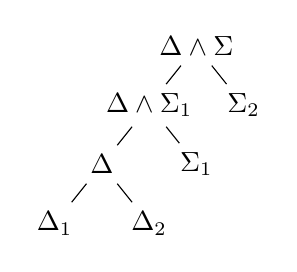
\begin{tikzpicture}[
            level distance=0.75cm,
            sibling distance=1.2cm,
            every node/.style={align=center}
        ]
            \node {$\Delta \land \Sigma$}
                child {
                    node {$\Delta \land \Sigma_1$}
                    child {
                        node {$\Delta$}
                        child { node {$\Delta_1$} }
                        child { node {$\Delta_2$} }
                    }
                    child { node {$\Sigma_1$} }
                }
                child { node {$\Sigma_2$} };
        \end{tikzpicture}
        \caption{Incremental}
    \end{subfigure}
    \hfill
    \begin{subfigure}{0.45\linewidth}
        \centering
        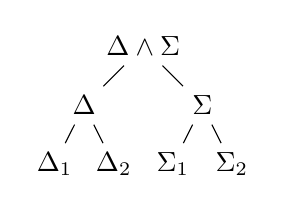
\begin{tikzpicture}[
            level distance=0.75cm,
            level 1/.style={sibling distance=1.5cm},
            level 2/.style={sibling distance=0.75cm}
        ]
            \node {$\Delta \land \Sigma$}
                child {
                    node {$\Delta$}
                    child { node {$\Delta_1$} }
                    child { node {$\Delta_2$} }
                }
                child {
                    node {$\Sigma$}
                    child { node {$\Sigma_1$} }
                    child { node {$\Sigma_2$} }
                };
        \end{tikzpicture}
        \caption{Non-incremental}
    \end{subfigure}

    \caption{Example of incremental and non-incremental approaches for compiling $\Delta \land \Sigma$.}
    \label{fig:compilation_comparison}
\end{figure}

\subsection{Preliminaries}

Before we present the Non-Incremental compilation algorithm, we contextualize the
results presented in the work of \citep{decolnet2023nonincremental}. First,
we define what we mean by \emph{Incremental Compilation} and \emph{Disjoint
Subsets} of a program.

\begin{definition}[Incremental Compilation]
    A bottom-up compilation of a boolean formula $\varphi$ is asequence
    $(\Sigma_1, I_1), \ldots, (\Sigma_N, I_N)$, where $\Sigma_1, \ldots,
    \Sigma_N$ are elements such that $\Sigma_N \equiv \varphi$
    and where, for every $i \in \{1, \ldots, N\}$, $I_i$ is an instruction
    telling how $\Sigma_i$ is obtained. Three types of instructions are
    possible:

    \begin{itemize}
        \item $\Sigma_i = \text{Compile}(c)$ for some constraint $c$ of
        $\varphi$. Then $\Sigma_i \equiv c$.
        \item $\Sigma_i = \text{Apply}(\Sigma_j, \Sigma_k, \land)$ for some
        $j, k < i$ such that $\Sigma_i, \Sigma_j, \Sigma_k$ respect the same
        vtree. Then $\Sigma_i \equiv \Sigma_j \land \Sigma_k$.
        \item $\Sigma_i = \text{Restructure}(\Sigma_j)$ for some $j < i$. Then
        $\Sigma_i \equiv \Sigma_j$ and their $V$-trees may differ.
    \end{itemize}
\end{definition}

\begin{lemma}[Lemma 13 \citep{decolnet2023nonincremental} \label{lemma:non_incremental}]
    Let $\phi_1$ and $\phi_2$ be such that $var(\phi_1) \cap var(\phi_2) =
    \emptyset$. Given $(D^1_1, I^1_1), \ldots, (D^1_s, I^1_s)$ an incremental
    $strDNNF(\land,r)$ compilation of $\phi_1$, and $(D^2_1, I^2_1), \ldots,
    (D^2_t, I^2_t)$ an incremental $strDNNF(\land,r)$ compilation of $\phi_2$,
    there is an incremental $strDNNF(\land,r)$ compilation of $\phi_1 \land
    \phi_2$ whose largest element has size at most $\max_i |D^1_i| + \max_j
    |D^2_j| + 1$.
\end{lemma}

Since SDDs are a subset of $strDNNF$ \citep{darwiche2011sdd}, it follows that
Lemma \ref{lemma:non_incremental} can be applied to $SDDs$.
Note that this Lemma \ref{lemma:non_incremental} presents an upper bound on the size
of the largest SDD obtained through the non-incremental compilation. In detail, by
choosing incremental compilations $\Delta = (D_1, I_1), \ldots, (D_n, I_n)$ and
$\Sigma = (S_1, J_1), \ldots, (S_m, J_m)$ of $\phi_1$ and $\phi_2$, respectively, we
can build a non-incremental compilation $(F_1, K_1), \ldots, (F_{n+m}, K_{n+m})$
of $\phi_1 \land \phi_2$ as follows:

\begin{itemize}
    \item $K_i = I_i$ and $F_i = D_i$ for $1 \leq i \leq n$.
    \item $K_{n+j} = J_j$ where every $S_j$ is replaced by $F_{n+j} = D_n
    \land S_j$. Thus, the root $F_{n+j}$ is and $\land$-node with children
    $D_n$ and $S_j$ (hence the size of $F_{n+j}$ is equal to $1 + |D_n| +
    |S_j|$).
\end{itemize}

Since $var(D_n) \cap var(S_j) \subseteq var(\Delta) \cap var(\Sigma) =
\emptyset$, each $F_{n+j}$ is a \textit{structured decomposable} circuit. Moreover,
it is a bottom-up compilation of $\phi_1 \land \phi_2$ whose size is at most
$\max(\max_i |D_i|, 1 + |D_n| + \max_j |S_j|)$.

\subsection{Non-Incremental Algorithm}

Suppose that a program $P$ can be decomposed into two disjoint sets of rules, $\phi_1$
and $\phi_2$, that do not share any variables. Incremental compilations for both
$\phi_1$ and $\phi_2$ exist, since we can compile both of them using the bottom-up
algorithm. Therefore, we can apply Lemma \ref{lemma:non_incremental} to obtain a
non-incremental compilation of $P$.

This is the core idea regarding the non-incremental compilation of $P$. If the program
$P$ is disjoint by nature, i.e. the dependency graph of $P$ has more than one connected
component, then we can identify such components through an algorithm such as Union-Find.
On the other hand, if $P$ is not disjoint by nature, we can apply a min-vertex-cut
algorithm to find a set of nodes that, when removed from the previous graph, will render
the graph disconnected into disjoint components, allowing application of the
non-incremental compilation. The only special consideration is that, after compiling the
disjoint components into a circuit $\Delta$, one also needs to compile the logical
constraints that were removed from the graph into another circuit $\Sigma$. The final
circuit representing the program $P$ is then obtained by conjoining $\Delta \land \Sigma$.

This process is summarized by the following theorem:

\begin{theorem}\label{theorem:non-incremental}
    Given a program $P$, we can determine $m$ disjoint subsets of the program in polynomial
    time, that can be non-incrementally compiled into a circuit of size at most $(m-1) +
    \sum_{i=1}^{m} |S_i|$, where $S_i$ is the size of the largest circuit obtained by
    compiling each subset using the bottom-up KC.
\end{theorem}

The result of this theorem is of special interest because usual conjoin (multiplication)
of SDDs is polynomial w.r.t. the size of the SDDs, but not linear. This multiplication
is indeed quadratic, bounded by the multiplication of the sizes of the two SDDs. Therefore,
having an upper bound that guarantees that the size of intermediary circuits will not
exceed the sum of the sizes of the individual circuits is highly desirable to avoid
exponential blow-up of intermediate circuits.

\begin{proof}[Proof of Theorem \ref{theorem:non-incremental}]\label{proof:non_incremental}
    First, it is possible to obtain $m$ disjoint subsets of head rules $\{c_1, \ldots,
    c_m\}$ of a program $P$ in polynomial time, by using an algorithm for
    $k$-vertex-connectivity (such as a min-vertex-cut algoritm).
    Next, we can compile the first set of head rules $r_i \in c_1$ into an SDD
    $\Delta$ by applying the bottom-up KC algorithm. Then we conjoin $\Delta$
    with the SDD $\Sigma_i$ representing the bottom-up compilation of each head rule
    $r_i \in c_2$, creating $k$ different ``clusters'' $\Delta \land \Sigma_i$ of SDDs
    \ref{fig:compilation_comparison}.

    Finally, we conjoin all these different clusters, obtaining an SDD with size at
    most $|S_1| + |S_2| + 1$ \ref{lemma:non_incremental}, where $|S_i|$ represents
    the size of the largest SDD obtained through an incremental compilation of the set
    of head rules in $c_i$, when following the bottom-up KC algorithm.

    This process can be repeated with the remaining components $c_3, \ldots, c_m$,
    resulting in an SDD of size at most $(m-1) + \sum_{i=1}^{m} |D_i|$.
\end{proof}

The above Proof \ref{proof:non_incremental} only regards the compilation of the
disjoint subsets of rules. As commented before, to obtain the correct semantics
of the original PASP program, it still is necessary to retrieve the rules removed
after the application of the min-vertex-cut algorithm, and conjoin them with the
circuit to obtain the desired compilation.

An interesting remark is that this non-incremental compilation could be applied to
the compilation of PLPs, since we only assume the structure of a dependency
graph. In reality, this approach is even more general due to Non-Incremental compilation
being a relatively novel concept, this is the first work that proposes a principled
approach to obtaining such disjoint components in order to utilize this approach in
practice.

\subsection{Preliminary Results}

Finally, we present a result similar to the one in Table~\ref{tab:vtree-comparison},
in the \textsc{Coloring} dataset with slower growth rate in graph sizes, but
comparing Non-Incremental and Incremental compilation. Figure~\ref{fig:non_inc}
highlights how the non-incremental compilation performed better not only in terms of
memory usage during compilation, but also in terms of compilation time. This results,
although unexpected at first glance, is due to the Non-Incremental approach being less
succeptible to the order of the rules that are being compiled, i.e. the order in which
we compile the Clark's completion has a great impact on the compilation time and
memory usage.

When first exploring both the Non-Incremental and Incremental compilation, the only optimization
that we proposed to the order in which rules of the Clark's completion are compiled was
to always prioritize the compilation of facts, as they are the most basic elements of the
knowledge base. After seeing the results of Fig~\ref{fig:non_inc}, we realized that
the heuristic proposed to generate good $V$-tree initializations should also be used to
guide the order in which rules are compiled. After applying the heuristic to the order
of the rules, we observed a significant improvement in the Incremental compilation time,
achieving similar performance as the Non-Incremental approach; and reducing the memory usage
considerably. Although the Non-Incremental approach still used less memory overall, we could see
that the memory usage difference for the largest instance of the \textsc{Coloring} dataset
fell from $0.6GB$ to $0.3GB$, still noticeable, but not as large as before.

Therefore, the Non-Incremental approach had three main impacts in this work: first, further improving
the incremental approach memory and time usage due to the aforementioned optimizations; second,
providing a more robust, less rule-ordering susceptible compilation; and third, providing a sound
approach for splitting a complex compilation problem into smaller, more manageable parts, that
can be easily parallelized without sacrificing performance due to encountering bad rule ordering.

\begin{figure}
    \centering
    \begin{subfigure}{0.48\linewidth}
        \centering
        \includegraphics[width=\linewidth]{../thesis/gfx/non_inc/coloring_time_non_inc.pdf}
        \caption{Compilation time (seconds).}
        \label{fig:non_inc_time}
    \end{subfigure}
    \hfill
    \begin{subfigure}{0.48\linewidth}
        \centering
        \includegraphics[width=\linewidth]{../thesis/gfx/non_inc/coloring_mb_non_inc.pdf}
        \caption{Peak memory usage (mb).}
        \label{fig:non_inc_mem}
    \end{subfigure}

    \caption{Comparison between incremental (y-axis) and non-incremental (x-axis)
    compilation as we increase the number of nodes (darker colors) of the graph
    \textsc{Coloring} program. The dotted black line represents the baseline; points
    above it indicate that the incremental approach performed worse.}
    \label{fig:non_inc}
\end{figure}

%---------------------------------------------------------------

\section{Discussion About Circuits}

Before advancing into the experimental results (Section~\ref{sec:experimental_results}),
we highlight the importance of compilation for Neuro-Symbolic systems and briefly cover
what remains to be addressed with respect to approximate compilation techniques.

\subsection{Learning the Circuit}

Another major advantage of using KC is the ability to
differentiate the weights of a circuit, which can be used as
the structure for a learning algorithm. This is particularly
useful when considering Neuro-Symbolic approaches, that
combine the Knowledge Representation of the program to define complex loss
functions over Neural Networks.

Therefore, the bottom-up compilation of the program
through the use of SDDs is not the last step for an
efficient PASP KC algorithm, as we discussed in this
section. It could also require a normalization step to obtain
the \textsc{MaxEnt} semantics (when using the \textit{smProblog}
approach); and, after that, differentiation can be done, to
learn both parameters of the circuit and Neural Networks acting as
\textit{annotated disjunctions}, through the use of gradient
descent \citep{geh2023dpasp, yang2023neurasp}.

Withal, advancements in the field of Probabilistic Circuits can be applied in
the learning of the circuit, such as regularization techniques
specifically designed for probabilistic circuits
\citep{liu2021tractable}.

\subsection{Partial Observations}

With inspiration from Problog 2 paper
\citep{fierens2015inference}, we also claim that there is the
possibility of compiling circuits w.r.t. certain queries.
The idea behind this approach is to only compile facts that are
associated with the query, and not the whole program.

This is a recurrent theme when only partial observations are
considered, and can act as a considerable \textit{speed-up} in
the overall inference routine. This is particularly useful when
considering the \textit{Neuro-Symbolic} approach, where not only
many queries are made, but they are repeated each epoch of the
learning algorithm.

Note that this approach can be particularly useful when
considering the \textit{smProblog} approach, since the removal
of facts that are not associated with the query can lead to a
more succinct circuit representation, which can alleviate the
enumerative step of the normalization algorithm.

\subsection{Approximate Compilation}

Approximate methods for compiling PLPs are a well-studied
topic, since the complexity of exact inference for these
languages is known to be intractable \citep{maua2020complexity}.
Thus, the possibility of using approximate methods for inference
(with or without KC is of great importance for the
development of the Neuro-Symbolic field.

Within this context, the work of \citep{pajunen2021solution} in ASEO and
\citep{manhaeve2021approximate} in \textit{DPLA} are both different methods, applied to
PASP and Problog programs, respectively, that aim to
circumvent the intractability associated with the exact
compilation of PLPs, by providing approximate methods for
inference (and, consequently, learning) of the parameters of the
program, with the tradeoff of not considering all possible
proofs of the query, but only the one with the highest
probability \citep{pajunen2021solution, manhaeve2021approximate}.

The first of these two methods, called ASEO, is based on
the concept of enumerating the $k$ most probable proofs of a
query, while the remaining ones are discarded and not
considered in the inference process \citep{pajunen2021solution}.
This process is done through the resolution of the homonymous
problem, ASEO, since it does not enumerate solutions, and
yet enumerate the most probable Answer Sets for a query (for an
example, the $k$ most probable that satisfy a literal $q$ and
evidence $e$) \citep{pajunen2021solution}. On the other hand,
the second method, \textit{DPLA}, is based on combining the
Selective Linear Definite (SLD) tree for best proof with the $A^*$ search, in order to
find the best proof (since the work only considered
\textit{stratified} programs, and, therefore, there is no need
to consider Answer Sets), the $k$ best proofs of a query or even
all proofs \citep{manhaeve2021approximate}.

In this sense, the work present in the literature contemplates
approximate methods for inference, with different approaches to
compilation in \textit{stratified} PLPs
\citep{vlasselaer2016tp, manhaeve2021approximate}. However,
approximate methods for PASP are still to be explored, as
only enumerative methods have been presented in the literature
\citep{pajunen2021solution}. Therefore, we believe that a
generalization of the $T_{C_\mathcal{P}}$ operator for general
Normal Logic Programs (instead of \textit{stratified} ones, as the
original work proposes) can be a promising approach for future
research in this area.

For example, by splitting a PASP program, through the
methods described in
\citep{lifschitz1994splitting, ben2021split}, into a
\textit{stratified} part and a \textit{non-stratified} part,
it would be possible to apply the $T_{C_\mathcal{P}}$ operator
on the former and PASP KC methods on the latter,
creating a hybrid approach for approximate inference by KC
in PASP. However, this is only a suggestion, and further
investigation is needed to determine the effectiveness of this
approach and to pursue further refinements.

%---------------------------------------------------------------

\section{Experimental Results}\label{sec:experimental_results}

This section wraps up the experimental results of our proposed methods
for Non-Incremental PASP KC, describing in further detail the
datasets chosen for evaluation, research questions, and some relevant
implementation considerations.

\subsection{Datasets}

Here, we describe each class of programs used in our experiments.
As opposed to other works on PASP KC, we focus on the
programs structure, and not their CNF representation.
Although this may seem quite intuitive, many previous works, such
as \citep{eiter2021treewidth, EITER2024104109, kiesel2023knowledge},
use CNF benchmarks as a proxy for PASP KC programs.
However, this approach has limitations, as it does not offer any
means to exploit program structure, which is crucial for our proposed
methods, both bottom-up KC or the $V$-tree heuristics.

In order to cope with these limitations, we propose using an extension
to the benchmark proposed by \citep{azzolini2024}. This benchmark has
two major drawbacks: the \textsc{Coloring} dataset is not consistent,
i.e. there are total choices without any models, which makes the whole
program probability less than $1$; and there are no cardinality
constraints. To address these issues, we introduce a new dataset called
\textsc{Food}, which models the problem of selecting an item from a menu,
given a distribution of preferences, subject to a majority vote on the
selected item.

\subsubsection{Coloring}

The \textsc{Coloring} dataset in Listing \ref{lst:coloring}, which models the
problem of coloring a graph with three colors is consistent, since we added
atoms $uncolorable$ and $colorable$, instead of using integrity constraints
that would throw away models. This dataset appears in two different versions
in our experiments:

\begin{enumerate}
    \item \textsc{Coloring}: where the edges were sampled from a random
    $G_{n,p}$ graph; and
    \item \textsc{Coloring Complete}: where the graph is complete.
\end{enumerate}

\begin{program}
    \begin{lstlisting}
    % Grounded Coloring Program
    0.5::edge(X, Y). % Probability of edge between nodes X and Y
    node(X). % Fact also derived from the dataset
    % A node can have only one of three colors
    red(X) :- node(X), not green(X), not blue(X).
    green(X) :- node(X), not red(X), not blue(X).
    blue(X) :- node(X), not red(X), not green(X).
    % Symmetry between edges
    e(X, Y) :- edge(X, Y).
    e(X, Y) :- edge(Y, X).
    % 3 graph coloring codification as
    uncolorable :- e(X, Y), red(X), red(Y).
    uncolorable :- e(X, Y), green(X), green(Y).
    uncolorable :- e(X, Y), blue(X), blue(Y).
    colorable :- not uncolorable.
    \end{lstlisting}
    \caption{Definition of the \textsc{Coloring} Dataset (class of programs).}
    \label{lst:coloring}
\end{program}

\subsubsection{PIN - Probabilistic Influence Network}

The \textsc{PIN} dataset in Listing \ref{lst:probabilistic_interaction_network}
models the dynamics of a disease spread across contact
network. Individuals can get infected either by contact with other \emph{infected}
individual of the network or by an external event (indicated by the
probabilistic predicate \emph{contaminated}). An infected individual might be
\emph{symptomatic} or not; non-symptomatic individuals are called \emph{vectors}
of the disease.

This type of network displays the typical transitivity closure often used to
evaluate logic program inferences (like the \textsc{Smokers} dataset
\citep{vlasselaer2014compiling}). Relative to the \textsc{Smokers} program, this
program also contains challenges relative to non-stratified negation and cyclic
dependencies, as the vector and symptomatic contradictory nature increase
considerably the complexity of the inference process, requiring $X$-determinism
to ensure tractability.

\begin{program}
    \begin{lstlisting}
    % Probabilistic Interaction Network (PIN)
    0.5::contaminated(1..N).
    0.5::friend(1..N, 1..N).
    infected(X) :- contaminated(X).
    infected(X) :- friend(X, Y), infected(Y).
    healthy(X) :- not infected(X).
    symptomatic(X) :- infected(X), not vector(X).
    vector(X) :- infected(X), not symptomatic(X).
    \end{lstlisting}
    \caption{Definition of the \textsc{PIN} (Probabilistic
    Influence Network) Dataset (class of programs).}
    \label{lst:probabilistic_interaction_network}
\end{program}

Similarly to the \textsc{Coloring} dataset, the \textsc{PIN} dataset has two versions:

\begin{enumerate}
    \item \textsc{PIN}: where the edges were sampled via snowball sampling on the
    Bitcoin OTC dataset \citep{kumar2016edge, kumar2018rev2}, a methodology similar
    to that of \citep{wang2020provenance}.
    \item \textsc{PIN Complete}: a complete graph.
\end{enumerate}

\subsubsection{IRL}\label{sec:irl}

The IRL dataset represents a sequence of probabilistic facts and logical rules.
It is designed to test the scalability of encoding techniques with respect to
the size of the body of the rules, with a fixed number of rules in the program.
It is a fairly simple dataset that acts a baseline and should, in theory,
behave especially well for top-down compilers, since there is no need to
introduce auxiliary variables in the Clark completion.

\begin{program}
    \begin{lstlisting}
    % IRL Problem
    0.5::a(1..N).
    qr :- a(X0), a(X2), a(X4), ..., a(Xeven).
    qr :- a(X1), a(X3), ..., a(Xodd), not nqr.
    nqr :- a(X1), a(X2), ..., a(Xn), not qr.
    \end{lstlisting}
    \caption{Definition of the \textsc{IRL} Dataset (class of programs).}
    \label{lst:irl}
\end{program}

\subsubsection{IRN}

For the IRN dataset \citep{azzolini2024}, we employed a similar strategy, varying the parameter $N$ from $1$ to $500$.

\begin{program}
    \begin{lstlisting}
    % IRN Problem
    0.5::a(1..N).
    qr :- a(Xeven).
    qr :- a(Xodd), not nqr.
    nqr :- a(Xodd), not qr.
    \end{lstlisting}
    \caption{Definition of the \textsc{IRN} Dataset (class of programs).}
    \label{lst:irn}
\end{program}

\subsubsection{N-Queens}

The N-Queens dataset models a probabilistic version of the classical N-Queens
problem, where queens must not attack each other. It demonstrates the
effectiveness of encoding techniques in handling spatial constraints. Due to
the high number of possible conflicts, it is expected that representing this
problem via a top-down approach will lead to quick blowups in circuit sizes.

For the $N$-Queens dataset in Listing \ref{lst:nqueens}, we have a probabilistic
version of the classical $N$-Queens problem, where each cell block can have a
queen with a certain probability. It demonstrates the
effectiveness of encoding techniques in handling spatial constraints. Due to
the high number of possible conflicts, it is expected that representing this
problem via a top-down approach will lead to quick blowups in circuit sizes.

\begin{program}
    \begin{lstlisting}
    rows(1..N). columns(1..N).
    % N-Queens Problem
    % For each cell block, there is a queen with a random
    % distribution over the columns.
    0.5::queen(R, C) :- rows(R), columns(C).
    % We encode both satisfiable and unsatisfiable instances
    % so there should always be a model
    conflict :- queen(R1, C1), queen(R2, C2), abs(R1 - R2) == abs(C1 - C2).
    conflict :- queen(R, C1), queen(R, C2), C1 != C2.
    conflict :- queen(R1, C), queen(R2, C), R1 != R2.
    \end{lstlisting}
    \caption{Definition of the \textsc{N-Queens} Dataset (class of programs).}
    \label{lst:nqueens}
\end{program}

\subsubsection{Food}

The Food dataset represents a preference selection problem, where the majority
needs to decide on an item to be selected (the type of food they will have).
This dataset is used to evaluate the impact of different encodings of cardinality
constraints including constraints other than ``exactly-one-of''.The number of
food items can be fixed in order to vary the number of people and, thus,
increasing only the cardinality constraints for the majority vote and annotated
disjunctions.

When creating instances of the \textsc{Food} dataset in Listing \ref{lst:food},
we kept the number of food items, $M$, constant as 4. This effectively fixed the
number of voting options and allowed us to study the effects of varying the
number of voters, $N$.

\begin{program}
    \begin{lstlisting}
    % Food Preference Problem
    % Define the domains of people and food
    person(1..N). food(1..M).
    % Annotated disjunctions encode preferences
    1/M::prefers(P,1); ...; 1/M::prefers(P,M) :- person(P).
    % Exactly one food type must be chosen
    1 { chosen(F) : food(F) } 1.
    % Someone agrees if their prefered food is chosen
    agrees(P) :- person(P), prefers(P,F), chosen(F).
    % Constraint: More than half must agree
    :- { P : agrees(P) } n//2.
    \end{lstlisting}
    \caption{Definition of the \textsc{Food} Dataset (class of programs).}
    \label{lst:food}
\end{program}

\subsection{Research Questions}

Finally, we conclude the chapter by revisiting all previous experiments
in a more unified manner, highlighting the strengths and limitations of
our proposed methods. We do this by summarizing the results obtained from
each experiment alongside its respective research question.

\begin{enumerate}
    \item \textbf{Research Question 1:} How the number of auxiliary atoms
    used to represent a program in CNF form scale?
    \item \textbf{Research Question 2:} Without any optimization, is the
    bottom-up KC algorithm competitive with other state-of-the-art
    algorithms?
    \item \textbf{Research Question 3:} Is the $V$-tree initialization
    heuristic better than other state-of-the-art heuristics?
    \item \textbf{Research Question 4:} Does the $V$-tree dynamic reordering
    offer a good trade-off between compilation time and circuit succinctness?
    \item \textbf{Research Question 5:} The proposed method for encoding
    cardinality constraints is competitive with other state-of-the-art
    methods constraint encoding techniques?
    \item \textbf{Research Question 6:} Is the price of imposing
    $X$-constrainedness too high?
    \item \textbf{Research Question 7:} Is the proposed non-incremental
    approach capable of avoiding large intermediate representations?
    \item \textbf{Research Question 8:} If we combine every possible
    optimization, can we achieve a significant improvement in compilation
    time and circuit succinctness, when compared to the state-of-the-art
    algorithms?
\end{enumerate}

First, we have that \textbf{Q1} is answered by Figure~\ref{fig:auxiliary},
which shows that, for every class of programs besides \textsc{IRL}, we have
a great increase in the number of auxiliary atoms as we increase instance
size. This is due to programs with transitive dependencies (or other types
of relationships) having a quadratic or even higher increase in the number
of auxiliary atoms as we increase instance size.

For \textbf{Q2}, we observe in Figure~\ref{fig:2amc} that the bottom-up,
although competitive in some scenarios, such as the \textsc{IRN},
\textsc{PIN Complete} and \textsc{Queens} datasets, still suffers on
the majority of datasets, having a small loss on the \textsc{IRL} dataset.
We can see that this change for datasets \textsc{IRL} and \textsc{Food}
when we consider dynamic minimization, as shown in Figure~\ref{fig:vtree}
(\textbf{Q4}). This is further enhanced by the $V$-tree initialization heuristic, which
significantly surpasses other CNF-based approaches, such as
\textsc{MinFill} or \textsc{MinDegree} (as shown in
Table~\ref{tab:vtree-comparison} - \textbf{Q3}).

Regarding different encodings of cardinality constraints, we observe that
they were essential to leverage the bottom-up compilation. When using
methods such as \textit{Sequential Counters} or \textit{Totalizers}, the
maximum instance sizes that the bottom-up approach was able to compile
were $13$ and $7$, respectively (even when using dynamic reordering). On
the other hand, by using the proposed method of this work, we were able
to not only avoid introducing auxiliary variables, but also were able to
compile up to $25$ instances. Larger instances could be compiled, but
generating such programs consumed more than the time wall of 30 minutes.
The displayed results in Figures \ref{fig:2amc}, \ref{fig:vtree},
\ref{fig:unconstrained} and \ref{fig:best} use the best encoding of
cardinality constraints for each compiler, i.e. \textit{Sequential Counters}
for \textsc{c2d} and \textit{Totalizers} for both \textsc{d4} and
\textsc{SharpSAT-TD}.

The limitations of imposing $X$-constrainedness were quite interesting,
as Figure~\ref{fig:unconstrained} shows (\textbf{Q6}). By imposing
$X$-constrainedness, the most impacted datasets were the ones where the
bottom-up approach had significantly worse performance than the top-down
approaches, \textsc{Coloring} and \textsc{PIN}. These datasets are
characterized by having a slower increase in the number of auxiliary
variables introduced as the problem size grows (as opposed to other
classes of programs such as \textsc{Food} or \textsc{Queens}, where the
growth is much faster). Thus, not imposing $X$-constrainedness can be an
interesting alternative for balancing compilation time, being able to
compile larger instances, but requiring post-processing to ensure the
correctness of the resulting circuit. On the other hand, an important
remark is that many KC libraries (such as the \textsc{SDD} package,
used for our approach) are not designed to handle more general Probabilistic Circuits
operations, which make it far from trivial to implement the complex
algorithm from \citep{zhang2025} (which does not have any implementation
available online). Therefore, the circuit sizes in Figure~\ref{fig:unconstrained}
are of unconstrained SDDs, and do not display the size of the
resulting circuit after applying the algorithm described in \citep{zhang2025}.

Finally, Figure~\ref{fig:non_inc} shows how the Non-Incremental can be
important to avoid larger intermediate circuit representations, which can
lead to increased compilation time and memory usage; or even incapacitate
compilation of certain instance sizes (\textbf{Q7}). This is further highlighted
by Figure~\ref{fig:best}, which shows a more consistent performance of the
bottom-up algorithm, alongside the Non-Incremental approach. By combining all
methods described in this thesis, the Non-Incremental method was capable of
producing smaller circuits than the top-down approach in most of the
considered datasets, even though we are imposing hard constraints, such
as $X$-constrainedness, during compile time (\textbf{Q8}).

\begin{figure}
  \centering
  \begin{subfigure}{0.48\linewidth}
    \centering
    \includegraphics[width=\linewidth]{../thesis/gfx/best/Vtree_irl.pdf}
    \caption{IRL}
    \label{fig:best_irl}
  \end{subfigure}
  \hfill
  \begin{subfigure}{0.48\linewidth}
    \centering
    \includegraphics[width=\linewidth]{../thesis/gfx/best/Vtree_irn.pdf}
    \caption{IRN}
    \label{fig:best_irn}
  \end{subfigure}
  \vspace{0.5em}
  \begin{subfigure}{0.48\linewidth}
    \centering
    \includegraphics[width=\linewidth]{../thesis/gfx/best/Vtree_coloring.pdf}
    \caption{Coloring}
    \label{fig:best_coloring}
  \end{subfigure}
  \hfill
  \begin{subfigure}{0.48\linewidth}
    \centering
    \includegraphics[width=\linewidth]{../thesis/gfx/best/Vtree_coloring_complete.pdf}
    \caption{Coloring Complete}
    \label{fig:best_coloring_complete}
  \end{subfigure}
  \vspace{0.5em}
  \begin{subfigure}{0.48\linewidth}
    \centering
    \includegraphics[width=\linewidth]{../thesis/gfx/best/Vtree_pin_best.pdf}
    \caption{PIN}
    \label{fig:best_pin}
  \end{subfigure}
  \hfill
  \begin{subfigure}{0.48\linewidth}
    \centering
    \includegraphics[width=\linewidth]{../thesis/gfx/best/Vtree_pin_complete_best.pdf}
    \caption{PIN Complete}
    \label{fig:best_pin_complete}
  \end{subfigure}
  \vspace{0.5em}
  \begin{subfigure}{0.48\linewidth}
    \centering
    \includegraphics[width=\linewidth]{../thesis/gfx/best/Vtree_food_best.pdf}
    \caption{Food}
    \label{fig:best_food}
  \end{subfigure}
  \hfill
  \begin{subfigure}{0.48\linewidth}
    \centering
    \includegraphics[width=\linewidth]{../thesis/gfx/best/Vtree_queens.pdf}
    \caption{Queens}
    \label{fig:best_queens}
  \end{subfigure}
  \caption{Comparison of circuit size for the Non-Incremental bottom-up
  compilation and top-down compilers across eight different datasets. The x-axis and y-axis
  represent, respectively, the size of the circuit produced by a compiler and the instance size.
  Cyan, magenta, yellow, and black represent, respectively: \textsc{c2d}, \textsc{d4}, \textsc{SharpSAT-TD}
  and the bottom-up SDD compiler with dynamic reordering. Datasets where the black dots
  are consistently under the other colors representing scenarios where the bottom-up SDD
  compiler is more efficient; and vice versa.}
  \label{fig:best}
\end{figure}
